%************************************************
\chapter{Image Decomposition}\label{ch:decomposition}
%************************************************

In this chapter, we will focus on those \ac{CAD} systems that use a combination of an image decomposition method and feature selection by means of hypothesis testing. These variety of methods have been published in \cite{Martinez201141,Martinez-Murcia20129676,Martinez-Murcia2013255,Martinez-Murcia201458}. 

Image decomposition methods model a set of samples as a linear combination of $c$ latent variables, also known as components. These variables can be considered as the basis of a $c$-dimensional space where each sample is represented by a feature vector of length $c$. The $i$-th neuroimage in our dataset can be therefore decomposed as: 

\begin{equation}\label{eq:generalDecomposition}
\mathbf{x}_i = s_0 \mathbf{w}_0 + s_1 \mathbf{w}_1 + \dots + s_c \mathbf{w}_c + \boldmath\epsilon = \mathbf{s}\mathbf{W} + \boldmath\epsilon
\end{equation}

Where $s_i$ is the coordinate (or component score) of the current image in the $i$-th dimension of the new space defined by all the base vectors $\mathbf{w}_i$ (component loadings), and $\boldmath\epsilon$ is the error of the estimation. Figure \ref{fig:decomposition_overview} shows an illustration of the process. 

\begin{figure}[tph]
	\centering
	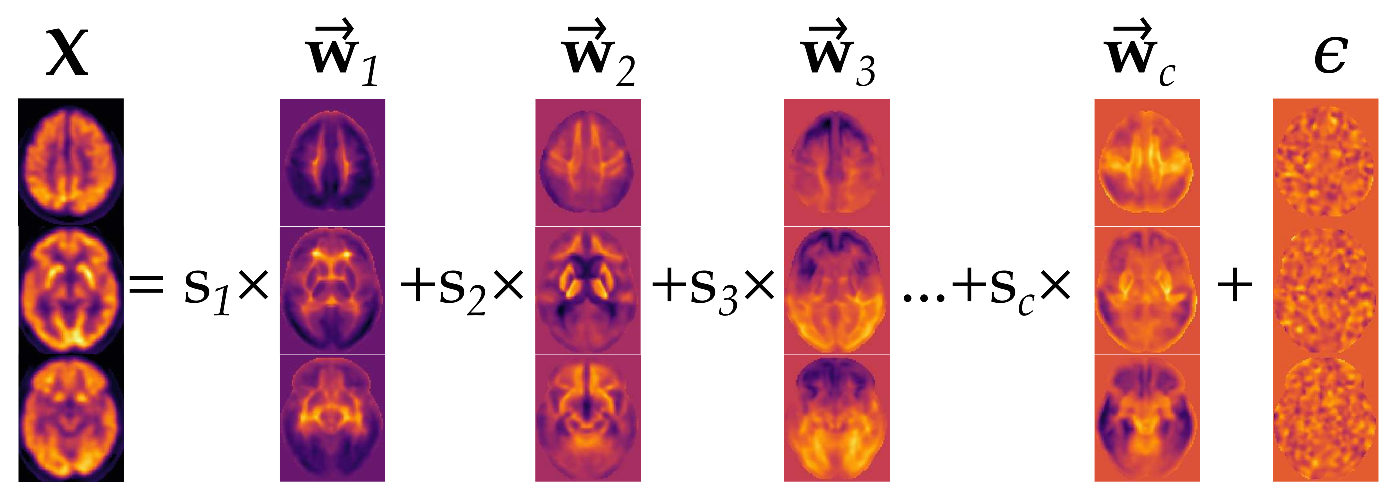
\includegraphics[width=0.9\linewidth]{Graphics/ch4/decomposition_overview}
	\caption[Illustration of how decomposition algorithms work.]{Illustration of how decomposition algorithms such as \ac{FA} and \ac{ICA} work on a \ac{PET}-FDG brain image.}
	\label{fig:decomposition_overview}
\end{figure}

Many signal decomposition techniques are used in the literature, for example \ac{PCA} or \ac{PLS} \cite{Spetsieris2009,Illan2011,Towey2011,Segovia2013,Khedher2015}. We will focus on two less known decomposition algorithms \acf{FA} and \acf{ICA}, which we will integrate in different \ac{CAD} systems using a pipeline similar to the one displayed at Figure~\ref{fig:pipelineDecomposition}. This pipeline involves feature selection (for reducing the dimensionality), decomposition of the feature vectors and classification.

\begin{figure}[tph]
	\centering
	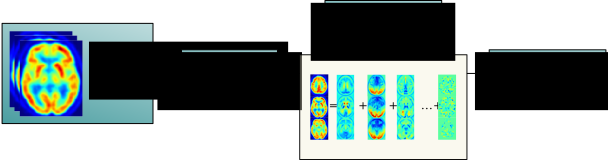
\includegraphics[width=0.9\linewidth]{Graphics/ch4/01-flowdiagram}
	\caption[Illustration of the system used in chapter~\protect\ref{ch:decomposition} .]{Illustration of the system used in chapter~\protect\ref{ch:decomposition}.}
	\label{fig:pipelineDecomposition}
\end{figure}

\section{Feature Selection}\label{sec:featureSelection}
Feature selection is the first strategy used for feature reduction \cite{Martinez-Murcia2016b}, and it is often used along with feature extraction in order to build more complex pattern recognition systems. It refers to any strategy intended to find a subset of the original features containing the more suitable ones according to a certain criterion. Therefore, irrelevant features are discarded, and resultant models are faster and more cost-effective \cite{Guyon03}. However, it usually requires an additional optimization to find the parameters for the optimal feature subset, and furthermore, it is impossible to guarantee that the optimal features for the subset are the same of the full feature set \cite{DaelemansHosteMeulderEtAl2003}. 

In this work, we will use filtering methods to perform feature selection. As we introduced in section~\ref{sec:mvanalyses}, filtering methods are based on the computation of a feature relevance score directly on the data. The relevance score is used to sort the different features, discarding those with a lower score, and it is usually computed independently for each feature, in what is called a univariate approach \cite{SaeysInzaLarranaga2007}. 

Feature selection can be used before or after feature extraction. When using computationally-intensive algorithms such as \ac{FA} or especially \ac{ICA}, the selection of best features prior to the decomposition is key to obtain high performance while keeping the computation times small \cite{Martinez201141,Martinez-Murcia20129676}. This also removes noise in some cases where the decomposition algorithm cannot compute correctly the variance. 

Three feature selection algorithms have been used in this thesis, not only in the \ac{CAD} systems proposed in this chapter, but in many other models that will be presented later: the $t$-Test, the Kullback-Leibler divergence or Relative Entropy, and the Mann-Whitney-Wilcoxon rank test. 

\subsection{$t$-test}\label{sec:ttestEq}
The $t$-test is an old friend of statisticians. In this work we will use the independent two-sample $t$-test \cite{Fay10}. It quantifies the differences between two classes using an assumption of independent variances. Let $X_i^f$ a vector containing the $f$-th feature of all elements in class $i$. The $t$-score of the $f$-th feature can be computed as:

\begin{equation}
t_f = \frac{\bar{X}_1^f - \bar{X}_2^f}{\sqrt{\frac{\sigma_{X_2^f}^2+\sigma_{X_1^f}^2}{n}}}
\end{equation}
where $\sigma_{X_i^f}^2$ is the variance and $\bar{X}_i^f$ is the average of the $f$-the feature within class $i$. The $t$-test is extensively used in the neuroimaging community, and it is the basis for the \ac{SPM} and \ac{VBM} analyses \cite{spm_book}. See figure~\ref{fig:ttest_map} for an example of the $t$-test computed on the \adnipet{} database.

\subsection{Kullback-Leibler Divergence} 
Another alternative is the \acf{KL} divergence, also known as Relative Entropy. It is a non-symmetric measure of the difference between two probabilities distributions. Let us assume that $X_1^f$ and $X_2^f$, the vectors containing the $f$-th feature of all elements in class $i$, are two discrete random variables. Therefore, the \ac{KL} divergence can be calculated with equation \ref{eq:kullback} \cite{Theodoridis1999}.

\begin{equation}\label{eq:kullback}
KL_f = \left(\frac{\sigma_{X_2^f}^2}{\sigma_{X_1^f}^2} +\frac{\sigma_{X_1^f}^2}{\sigma_{X_2^f}^2} -2 \right) + \frac{1}{2}\left(\bar{X}_2^f-\bar{X}_1^f\right)^2\left(\frac{1}{\sigma_{X_1^f}^2} + \frac{1}{\sigma_{X_2^f}^2}\right)
\end{equation}
using the same notation than in $t$-test. See figure~\ref{fig:kl_map} for an example of the computed \ac{KL} divergence on the \adnipet{} database.

\subsection{Mann-Whitney-Wilcoxon} 
The \acf{MWW} rank test, also known as $U$-test, assigns a rank to all values in the vector corresponding to the $f$-th feature, $X^f$, without considering any class. The method used to assign a rank is the `average', which means that each value is assigned with the average of the ranks that would have been assigned to all the tied values. This means that, for example, in the case of the vector $X^f=(0,2,3,2)$, the ranks assigned to each element would be $R^f=(1,2.5,4,2.5)$. 

Let $n_1$ and $n_2$ be the number of elements in class 1 and 2 respectively, and $R^f$ the vector of ranked elements. We proceed by selecting the first $n_1$ elements in $R^f$ by: 
\begin{equation}
R^f_{n_1} = {R^f_i} \quad \forall i\in(0,n_1)
\end{equation}

The $U$-score for the $f$-th feature and the first class will be: 
\begin{equation}
U_1^f = n_1 n_2 + n_1 \frac{n1+1}{2} - \sum R^f_{n_1}
\end{equation}

And the it can be computed for the second class as the remainder: 
\begin{equation}
U_2^f = n_1 n_2 - U_1
\end{equation}

The final $U^f$ can be assigned to either $U_1^f$, $U_2^f$ or $\min{U_1^f,U_2^f}$ \cite{Fay10}, but the usual approach nowadays is to assign $U^f=U_2^f$. Unlike $t$-test, \ac{MWW} test does not assume any prior distribution, and therefore is less likely than it to spuriously indicate significance because of the presence of outliers. Under the normal distribution, it performs relatively similar \cite{Fay10}. See figure~\ref{fig:wilcoxon_map} for an example of the \ac{MWW} $U$-test computed on the \adnipet{} database.

\section{Decomposition Algorithms}
The feature selection algorithms presented above will perform a significant feature reduction, from hundreds of thousands of voxels to a few thousands. These few thousands voxels are considered the best in discriminating between \ac{CTL} and affected subjects in each of the diseases. The feature selection strategy can be thought of as a mask, in which only the most relevant regions according to the tests are selected (see Figure~\ref{fig:comparisonSelection_adnipet}). 

However, this number of features is still large, and therefore, further feature reduction can be applied by performing a decomposition of the masked regions. We have used two algorithms in our \ac{CAD} systems: \acf{FA} and \acf{ICA}.

\begin{figure}[bth]
	\myfloatalign
	\subfloat[Original]
	{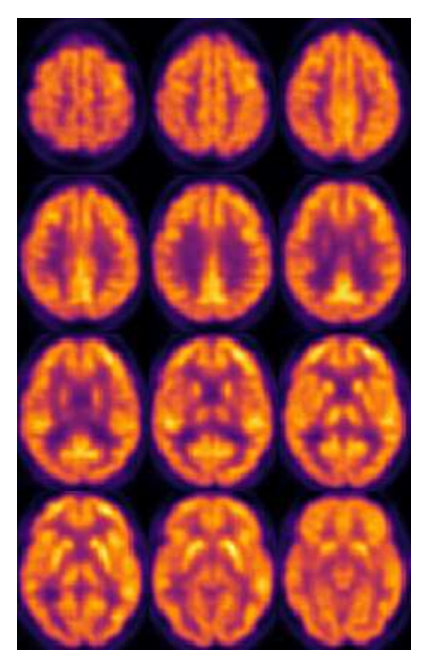
\includegraphics[width=.3\linewidth]{Graphics/ch4/originalImage_inferno.eps}}\quad
	\subfloat[\ac{FA} reconstruction]
	{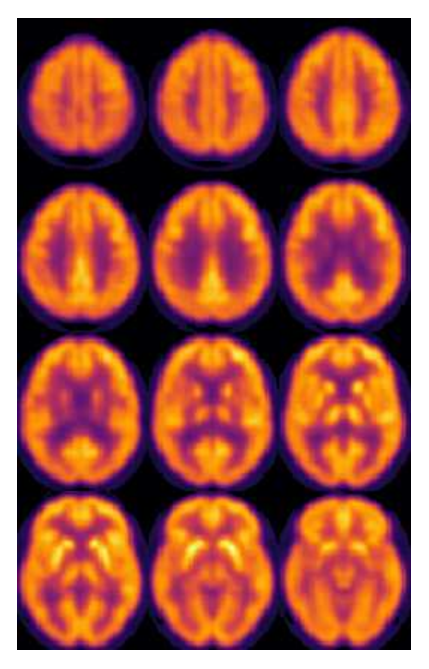
\includegraphics[width=.3\linewidth]{Graphics/ch4/transformedFA_inferno.eps}\label{fig:reconstructionFA}}\quad
	\subfloat[\ac{ICA} reconstruction]
	{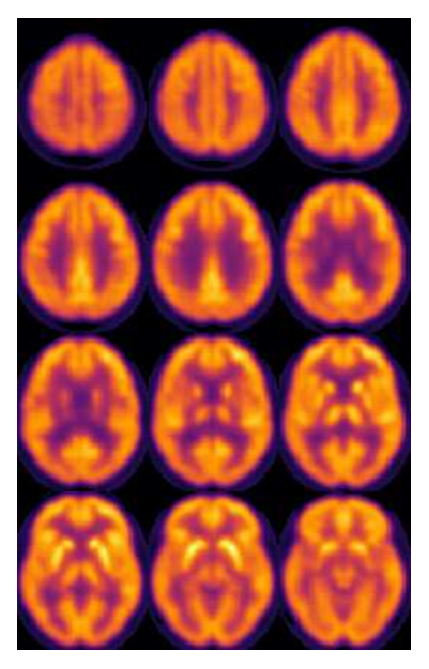
\includegraphics[width=.3\linewidth]{Graphics/ch4/transformedICA_inferno.eps}}
	\caption[Original \acs{PET} image and its reconstruction using FA or ICA.]{Original \acs{PET} image from the \adnipet{} dataset, and examples of reconstruction using \ac{FA} or \ac{ICA}, with 10 components.}\label{fig:comparisonReconstructions}
\end{figure}


\subsection{Factor Analysis}
\acf{FA} was used in \cite{Martinez201141,Martinez-Murcia20129676} to perform feature extraction in \ac{CAD} systems. This strategy assumes that each image in the database is a realization of a given experiment. \ac{FA} then models each of the $N$ observations (or subjects) as the expression of $c$ unobserved variables, known as factors. The model follows the general decomposition equation (Eq. \ref{eq:generalDecomposition}), but assuming that the dataset matrix $\mathbf{X}$ is zero-centred. That is, that we have subtracted the mean prior to the computation. In matrix form, Eq. \ref{eq:generalDecomposition} can be rewritten as:

\begin{equation}\label{eq:factoranalysis}
\mathbf{X} -\boldsymbol{\mu}= \mathbf{S}\mathbf{W} +  \boldsymbol{\epsilon}
\end{equation}

The columns of $\mathbf{W}$ are known as factors, and the rows of $\mathbf{S}$ are known as loadings  (similar to the concept of component loading and component scores in \ac{PCA}). Thanks to this, we can convert the original dataset $\mathbf{X}$ of size $N\times f$ into $\mathbf{S}$, of size $N\times c$. The procedure of computing the decomposition imposes some assumptions on $\mathbf{W}$: 
\begin{itemize}
	\item $\mathbf{W}$ and $\boldsymbol{\epsilon}$ must be independent. 
	\item $E[\mathbf{W}] = 0$. 
	\item $\text{Cov}(\mathbf{W}) = \mathbf{I}$, which ensures that the factors are uncorrelated. 
\end{itemize}

Now we can rewrite Eq.~\ref{eq:factoranalysis} as:
\begin{equation}\label{eq:fastep1}
\text{Cov}(\mathbf{X} -\boldsymbol{\mu})= \text{Cov}(\mathbf{S}\mathbf{W} +  \boldsymbol{\epsilon})
\end{equation} 

Under the previous constraints, and setting $\boldsymbol{\Sigma} = \text{Cov}(\mathbf{X} -\boldsymbol{\mu})$, Eq.~\ref{eq:fastep1} becomes:
\begin{equation}
\boldsymbol{\Sigma} = \mathbf{S}\text{Cov}(\mathbf{W})\mathbf{S}^T - \text{Cov}(\boldsymbol{\epsilon})
\end{equation}

Since $\text{Cov}(\mathbf{W}) = \mathbf{I}$, and making $\text{Cov}(\boldsymbol{\epsilon})=\boldsymbol{\Psi}$, the diagonal matrix containing the specific variances of the reconstruction error, we obtain the alternative form of \ac{FA}: 
\begin{equation}
\boldsymbol{\Sigma} = \mathbf{S}\mathbf{S}^T - \boldsymbol{\Psi}
\end{equation}

The mean $\boldsymbol{\mu}$, and the matrices $\mathbf{S}$ and $\boldsymbol{\Psi}$ are obtained via Maximum Likelihood estimation. To guarantee an unique solution, we impose that $\mathbf{S}^T\boldsymbol{\Psi}^{-1}\mathbf{S}$ is a diagonal matrix. Then, we obtain the parameters by maximizing the log-likelihood given by the following expression: 
\begin{equation}
\ell(\mu,\mathbf{S},\boldsymbol{\Psi}) = - \frac{np}{2}\log{2\pi}- \frac{n}{2}\log{\left|\mathbf{SS}^T + \boldsymbol{\Psi}\right|} - \frac{1}{2}\sum_{i=1}^{n}(\mathbf{x}_i-\mu)^T(\mathbf{SS}^T+\boldsymbol{\Psi})(\mathbf{x}_i-\mu)
\end{equation} 

\ac{FA} differs from \ac{PCA} mainly because it performs an estimation of the noise, and needs the number of factors $c$ as an input. Choosing $c$ is not a naive task. A large $c$ can yield a small reconstruction error, but the factors will not be representative enough, leading to overfitting of the subsequent model. Conversely, a small $c$ can lead to a large reconstruction error, causing information loss. We have computed the reconstruction error variance over the \adnipet{} dataset, and plotted it in Figure~\ref{fig:error} (similar graphs can be obtained for other databases. This proves that the error is assymptotical as we increase $c$, and therefore, once arrived at certain error, the improvements are not significant. To observe how the error affects the reconstruction, in Figure~\ref{fig:reconstructionFA} we can compare a reconstructed image with its corresponding original. 

\begin{figure}[ht]
	\centering
	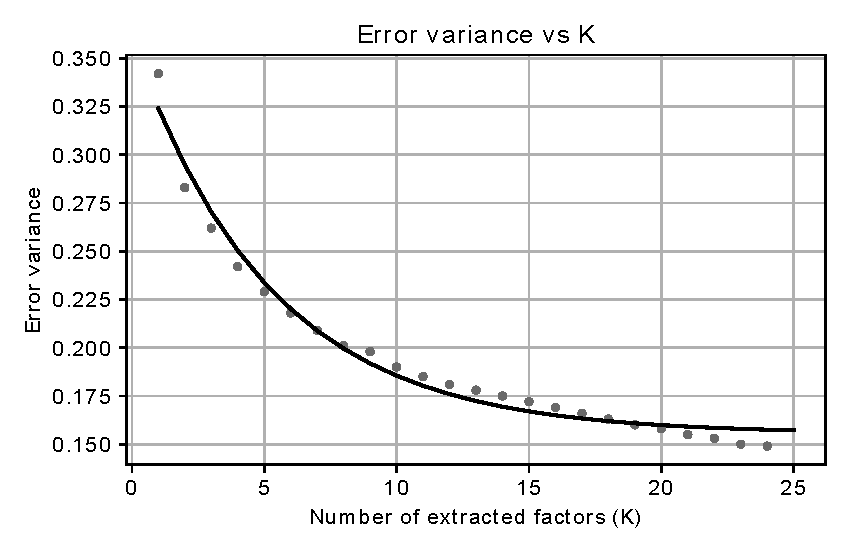
\includegraphics[width=0.5\linewidth]{Graphics/ch4/varError-K-ADNI}
	\caption[Variance of reconstruction error in \acs{FA}.]{Specific variance of reconstruction error $\Psi$ using \ac{FA}, in function of number of factors extracted ($K$) for \adnipet{} database (the behaviour is similar in other datasets).}
	\label{fig:error}
\end{figure}

\subsection{Independent Component Analysis}
\acf{ICA} \cite{Hyvarinen2000} is an algorithm that performs decomposition imposing that the resulting components must be independent. It was used in \cite{Alvarez2009,Martinez201141,Martinez-Murcia20129676} as part of a \ac{CAD} system, and it had been used in other medical imaging applications such as segmentation \cite{DeMartino2007}. 

\ac{ICA} was born as a solution to the \textit{blind source separation} problem, in which the aim is to estimate $c$ independent sources from a series of mixed signals \cite{Hyvarinen2000}. To do so, we assume the source signals to be non-gaussian, in addition to the independence assumption that we mentioned before. That is why their authors consider \ac{ICA} to be a non-gaussian version of \ac{FA} \cite{Hyvaerinen2003}, although due to this assumption, the results are very different to those obtained in \ac{FA}. 

Unlike \ac{FA}, \ac{ICA} does not account for noise in the estimation procedure, and therefore the equation remains: 
\begin{equation}\label{eq:icaecuation}
\mathbf{X} = \mathbf{W}\mathbf{S}
\end{equation}
where $\mathbf{S}$ are the component scores and $\mathbf{W}$ are the component loading, `sources' or `mixing matrix'. Given that \ac{ICA} lacks a noise term, there is a procedure called \textit{whitening} that must be applied for the algorithm to converge \cite{Hyvarinen2000}. The whitening implies a linear transformation of the $i$-th observed variable $\mathbf{x}_i$ into a \textit{white} vector $\tilde{\mathbf{x}}_i$ so that its covariance matrix equals the identity: 

\begin{equation}
E\{\tilde{\mathbf{x}}_i \tilde{\mathbf{x}}_i^T\}=\mathbf{I}
\end{equation}

This procedure is often performed using the \acf{EVD} of the covariance matrix $E\{\mathbf{x}_i \mathbf{x}_i^T\} = \mathbf{E}\mathbf{D}\mathbf{E}^T$. $\mathbf{E}$ is the covariance matrix containing the eigenvectors of $E\{\mathbf{x}_i \mathbf{x}_i^T\}$, and $\mathbf{D}$ is a diagonal matrix whose diagonal elements are the eigenvalues of $E\{\mathbf{x}_i \mathbf{x}_i^T\}$. Whitening is done using the following equation: 

\begin{equation}
\tilde{\mathbf{x}}_i= \mathbf{E}\mathbf{D}^{-1/2}\mathbf{E}^T\mathbf{x}_i
\end{equation}

This procedure transform the mixing matrix to:
\begin{equation}
\tilde{\mathbf{x}}_i = \mathbf{E}\mathbf{D}^{-1/2}\mathbf{E}^T \mathbf{W}\mathbf{s}_i
\end{equation}
which is indeed orthogonal, as can be seen here:
\begin{equation}
E\{\tilde{\mathbf{x}}_i\tilde{\mathbf{x}}_i^T\} = \tilde{\mathbf{W}} E\{\tilde{\mathbf{s}}_i\tilde{\mathbf{s}}_i^T\}\tilde{\mathbf{W}}^T 	=\tilde{\mathbf{W}}\tilde{\mathbf{W}}^T=\mathbf{I}
\end{equation}

This property reduces the number of parameters to be estimated, since an orthogonal matrix contains $n(n-1)/2$ degrees of freedom, in contrast to the $n^2$ degrees of freedom of the original mixing matrix $\mathbf{W}$. 

Thanks to the central limit theorem, we assume that the sum of a large number of independent random variables tends will be approximately normally distributed, regardless of the individual statistical distributions \cite{Rice2006}. This property is used to maximize non-gaussianity and independence in the sources using any independence criteria such as the kurtosis or negentropy in any of the proposed algorithms. In this work, we will use the FastICA algorithm. 

\subsubsection{FastICA}
FastICA is a block fixed-point iteration algorithm \cite{Oja1997,FastICA99} based on negentropy as a non-gaussianity measure. Fixed-point algorithms are converge faster than adaptive algorithms \cite{FastICA99}. The FastICA algorithm can be considered a neural algorithm \cite{Hyvarinen2000}, where the weight vector $\mathbf{w}$ can be updated using a learning rule. FastICA defines a learning rule that finds a direction $\mathbf{w}$, a unit vector such that the projection $\mathbf{w}^T\mathbf{x}_i$ maximizes non-gaussianity \cite{FastICA99}. 

The non-gaussianity measure used here is the negative entropy, or negentropy. The negentropy is a form of differential entropy, which for a random vector $\mathbf{y}$ is defined as: 
\begin{equation}
J(\mathbf{y})=H(\mathbf{y}_{gauss})-H(\mathbf{y})
\end{equation}
where  $\mathbf{y}_{gauss}$ and $\mathbf{y}$ share the same covariance matrix, although $\mathbf{y}$ is not a gaussian random variable, and $\mathbf{y}_{gauss}$ is. There are many approximations to negentropy. The FastICA defines negentropy using the function: 
\begin{equation}
J(y)\propto [E\{G(y)\}-E\{G(\nu)\}]^2
\end{equation}
where we assume that $y$ is of zero mean and unit variance, $\nu$ is a Gaussian variable sharing the same mean and variance, and $G(x)$ is any non-quadratic function. Many functions have been proposed, but in the FastICA algorithm we use either $G(x)_1 = (1/a_1) \log\cosh a_1 x$ with $1<a_1<2$ or $G(x)_2 = \exp(-x^2/2)$ \cite{FastICA99}. 

With these measures, we can compute the derivatives of these functions by: 
\begin{align}
g_1(x) & =\tanh(a_1 x), \\
g_2(x) & = x\exp(- x^2/2)
\end{align} 

The algorithm for the one-unit version of FastICA can be defined \cite{FastICA99} as:
\begin{enumerate}
	\item Choose an initial (e.g. random) weight vector ${\bf w}$.
	\item Let  ${\bf w}^+=E\{{\bf x}g({\bf w}^T{\bf x})\}-E\{g'({\bf w}^T{\bf x})\}{\bf w}$
	\item Let  ${\bf w}={\bf w}^+/\Vert{\bf w}^+\Vert$
	\item If not converged, go back to 2.
\end{enumerate}

The algorithm considers that the values of $\mathbf{w}$ converge when their dot product is close to 1, that is, they are pointing in the same direction. Note that the expectations are computed as the sample mean in the FastICA algorithm. Additional modifications were presented in \cite{Hyvarinen2000}, in which step 2 is converted to a Newton iteration and further simplification is performed. 

This is the algorithm for one computational unit, or neuron, which computes one component. However, the procedure can be extended to $c$ components by defining $c$ neurons with weight vectors ${\bf w}_1,...,{\bf w}_c$ so that $\mathbf{W} = ({\bf w}_1,...,{\bf w}_n)^T$. The outputs ${\bf w}_1^T{\bf x},...,{\bf w}_n^T{\bf x}$ must be decorrelated to prevent them from converging to the same maxima, using three methods proposed in \cite{Hyvarinen2000}. 

The method used in this work uses a two-step iterative algorithm \cite{Hyvarinen2000} to decorrelate the outputs after each iteration: 
\begin{enumerate}
	\item Let $\mathbf{W} = \mathbf{W}/\sqrt{\lVert\mathbf{W}\mathbf{W}^T\rVert}$. 
	\item Let $\mathbf{W} = \frac{3}{2} \mathbf{W}-\frac{1}{2} \mathbf{W} \mathbf{W}^T  \mathbf{W}$
\end{enumerate}

And repeat step 2 until convergence. For simplicity, the norm in step 1 can be computed as any norm but the Frobenius norm, for example, the L2-norm or the largest absolute row sum. 

\section{Results}
In this work we will analyse the behaviour of the system proposed in the introduction and illustrated at Figure~\ref{fig:pipelineDecomposition}. The system comprises the selection of the most relevant voxels using filtering methods (we will focus on $t$-test, relative entropy and wilcoxon) and a feature decomposition of these using either \ac{FA} or \ac{ICA}. Finally, the feature vectors are classified using a \ac{SVC} with linear kernel, and performance values are obtained via cross-validation (see section~\ref{sec:validation} for more information). 

We vary the number of selected voxels and the number of factors or components depending on the algorithm and the dataset used and evaluate the system with those characteristics. That way, we obtain an estimation of the performance of the system in different situations, so that we can draw conclusions on the disease patterns and the ability of the system in the detection of different diseases. 

\subsection{Alzheimer's Disease}
We begin by applying the proposed feature selection plus decomposition pipeline to the two functional neuroimaging datasets: \adnipet{} and \vdlnhmpao{}. For this experiment we will use a maximum of $20,000$ selected voxels and $25$ components. 

\subsubsection{Factor Analysis}\label{sec:results_FA_AD}
First, we use \ac{FA} as a decomposition technique. In Figure~\ref{fig:accuracyMeanFA-AD} we average the accuracy over the number of voxels or the number of components respectively, to look at how these variables affect the performance of the system, and we do this for the three filtering methods used. 

\begin{figure}	\centering
	\subfloat[]{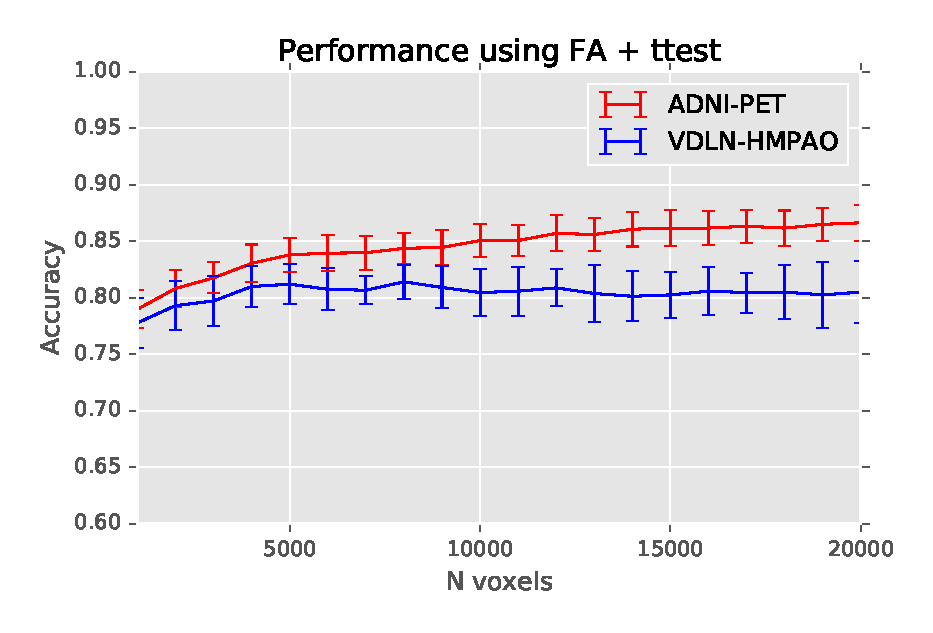
\includegraphics[width=0.49\linewidth]{Graphics/ch4/accuracyMeanSTD-FA_vsN_ttest_AD.eps}\label{fig:AD-AV-FA-TTEST-VSN}}
	\subfloat[]{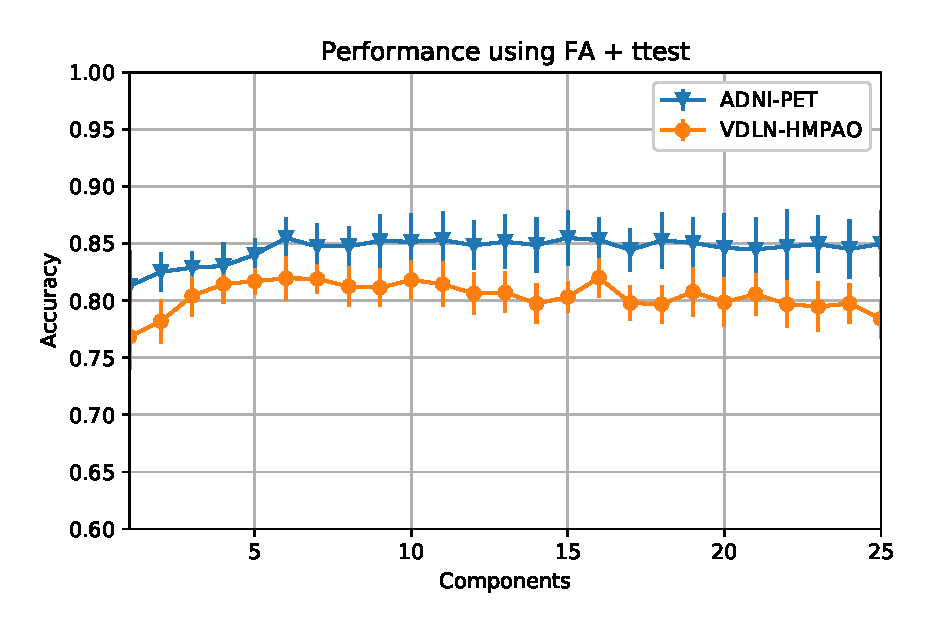
\includegraphics[width=0.49\linewidth]{Graphics/ch4/accuracyMeanSTD-FA_vsK_ttest_AD.eps}\label{fig:AD-AV-FA-TTEST-VSK}}
	
	\subfloat[]{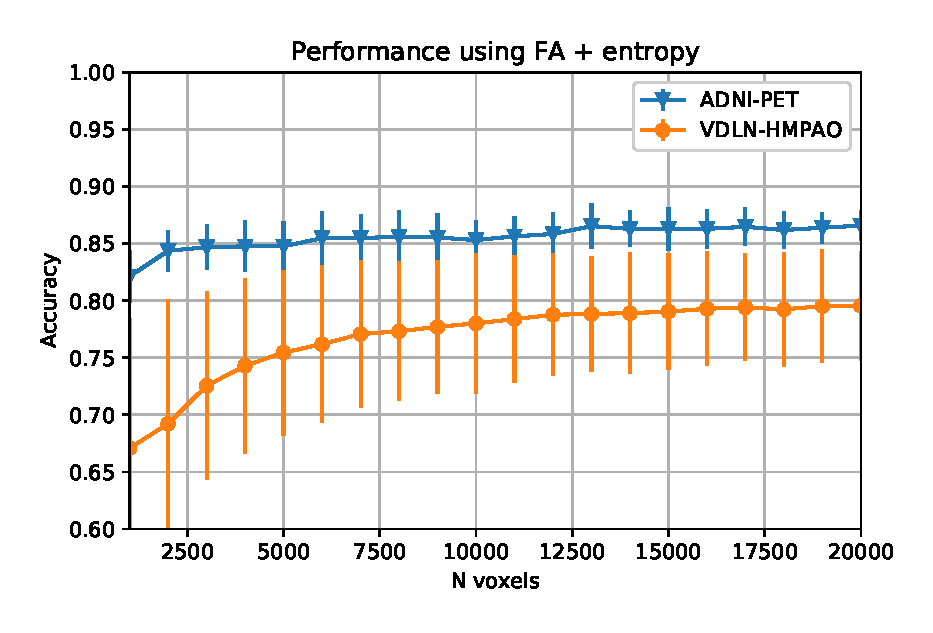
\includegraphics[width=0.49\linewidth]{Graphics/ch4/accuracyMeanSTD-FA_vsN_entropy_AD.eps}\label{fig:AD-AV-FA-ENTROPY-VSN}}
	\subfloat[]{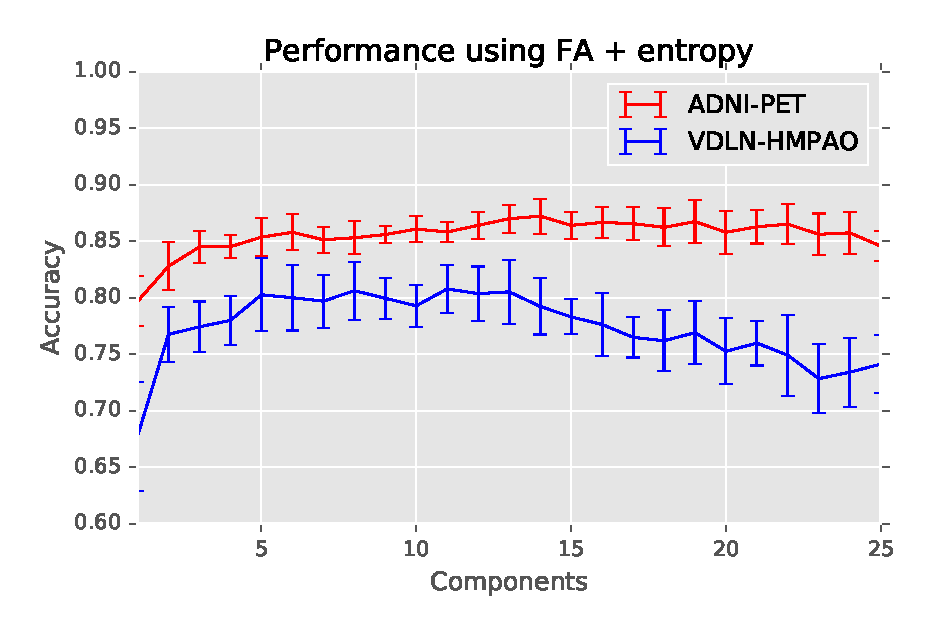
\includegraphics[width=0.49\linewidth]{Graphics/ch4/accuracyMeanSTD-FA_vsK_entropy_AD.eps}\label{fig:AD-AV-FA-ENTROPY-VSK}}
	
	\subfloat[]{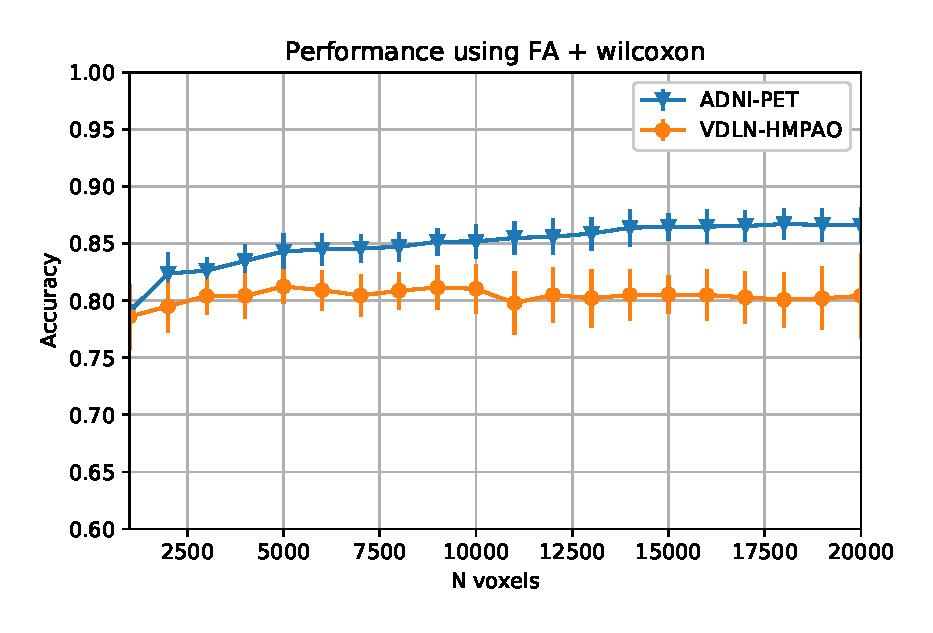
\includegraphics[width=0.49\linewidth]{Graphics/ch4/accuracyMeanSTD-FA_vsN_wilcoxon_AD.eps}\label{fig:AD-AV-FA-WILCOXON-VSN}}
	\subfloat[]{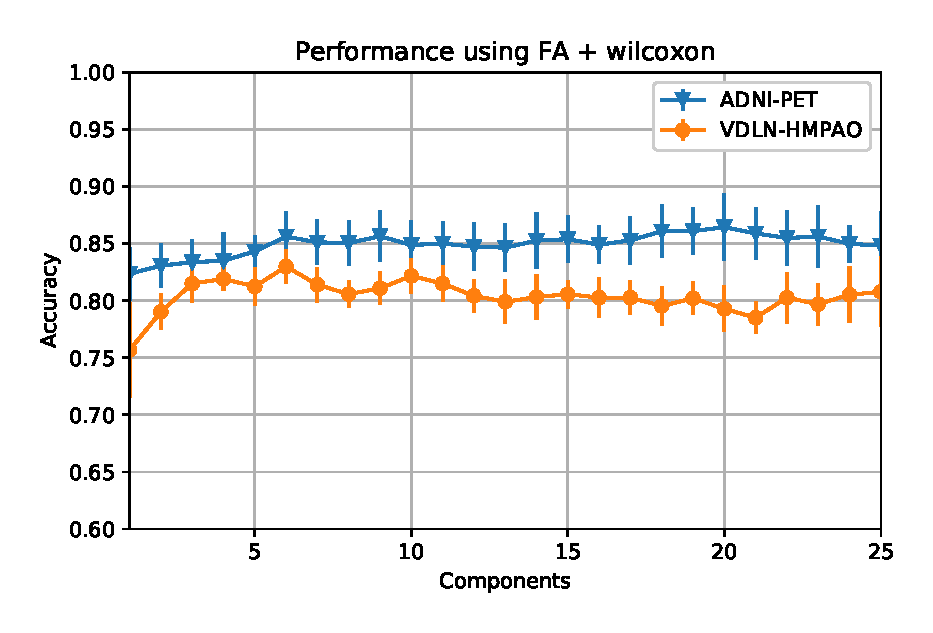
\includegraphics[width=0.49\linewidth]{Graphics/ch4/accuracyMeanSTD-FA_vsK_wilcoxon_AD.eps}\label{fig:AD-AV-FA-WILCOXON-VSK}}
	
	\caption[Average performance of the \acs{AD} datasets in \acs{FA}.]{Average performance and standard deviation of the proposed system using the two \ac{AD} datasets, \ac{FA} and the three feature selection criteria: $t$-test (\protect\subref{fig:AD-AV-FA-TTEST-VSN} and \protect\subref{fig:AD-AV-FA-TTEST-VSK}), relative entropy (\protect\subref{fig:PKS-AV-FA-ENTROPY-VSN} and \protect\subref{fig:AD-AV-FA-ENTROPY-VSK}) and wilcoxon (\protect\subref{fig:AD-AV-FA-WILCOXON-VSN} and \protect\subref{fig:AD-AV-FA-WILCOXON-VSK}). } 
	\label{fig:accuracyMeanFA-AD}
\end{figure}

We can observe that the results are generally better when using the \adnipet{} dataset than with the \vdlnhmpao{}, and this is especially notorious when using the relative entropy selection criterion. The performance tends to slightly increase with the number of voxels selected, but it is not the case with the number of components. By looking at figures \ref{fig:AD-AV-FA-TTEST-VSK}, \ref{fig:AD-AV-FA-ENTROPY-VSK} and \ref{fig:AD-AV-FA-WILCOXON-VSK}, it seems that a relatively small number of components (approximately 6) is enough to obtain good performance, and afterwards, the performance holds or even decreases. 

\subsubsection{Independent Component Analysis}
In this section, we compute the results of applying \ac{ICA} to the \adnipet{} and \vdlnhmpao{} datasets. Figure~\ref{fig:accuracyMeanICA-AD} depicts the average accuracy over the number of voxels or the number of components respectively for the different selection criteria. 

\begin{figure}
	\centering
	\subfloat[]{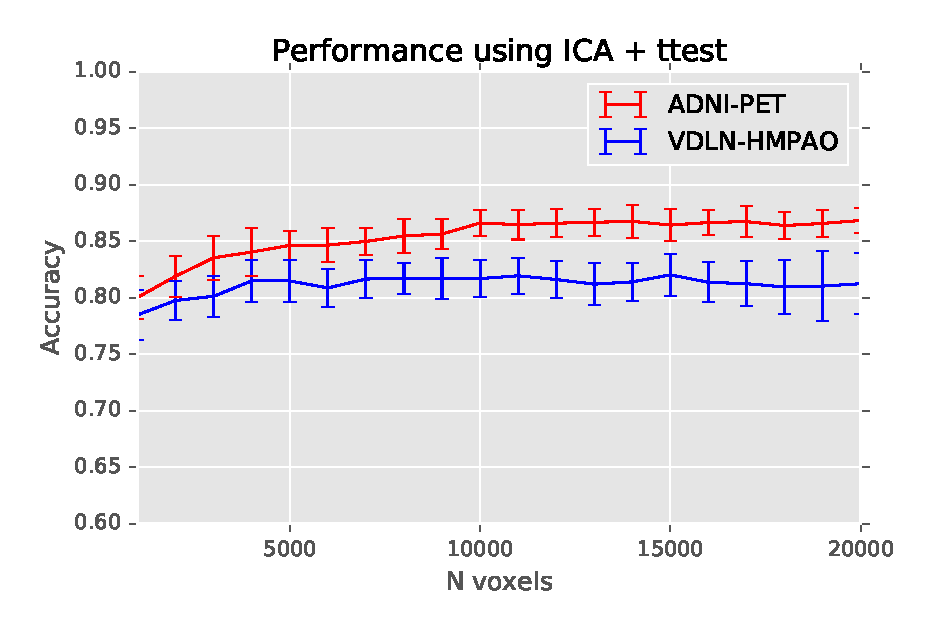
\includegraphics[width=0.49\linewidth]{Graphics/ch4/accuracyMeanSTD-ICA_vsN_ttest_AD.eps}\label{fig:AD-AV-ICA-TTEST-VSN}}
	\subfloat[]{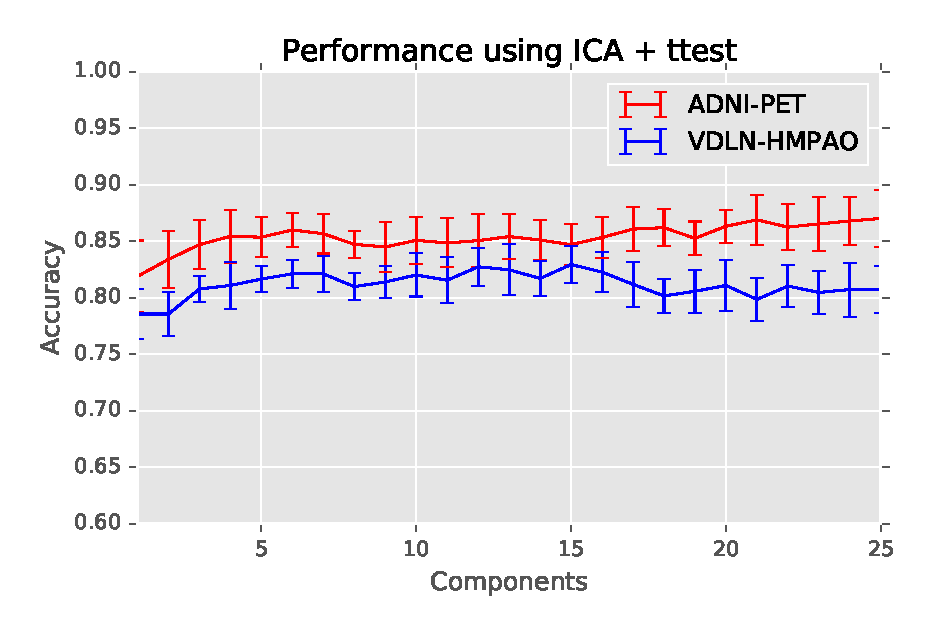
\includegraphics[width=0.49\linewidth]{Graphics/ch4/accuracyMeanSTD-ICA_vsK_ttest_AD.eps}\label{fig:AD-AV-ICA-TTEST-VSK}}
	
	\subfloat[]{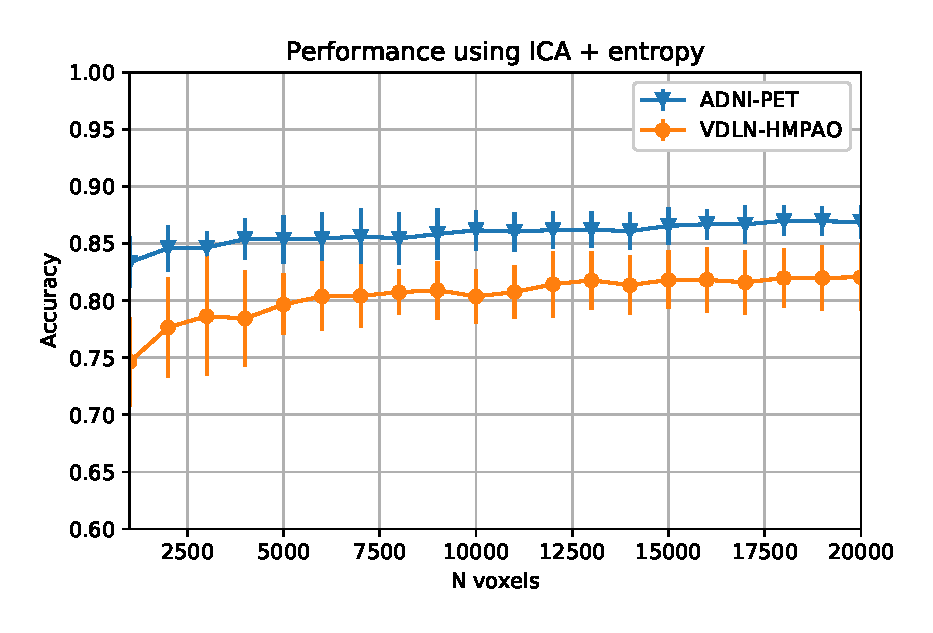
\includegraphics[width=0.49\linewidth]{Graphics/ch4/accuracyMeanSTD-ICA_vsN_entropy_AD.eps}\label{fig:AD-AV-ICA-ENTROPY-VSN}}
	\subfloat[]{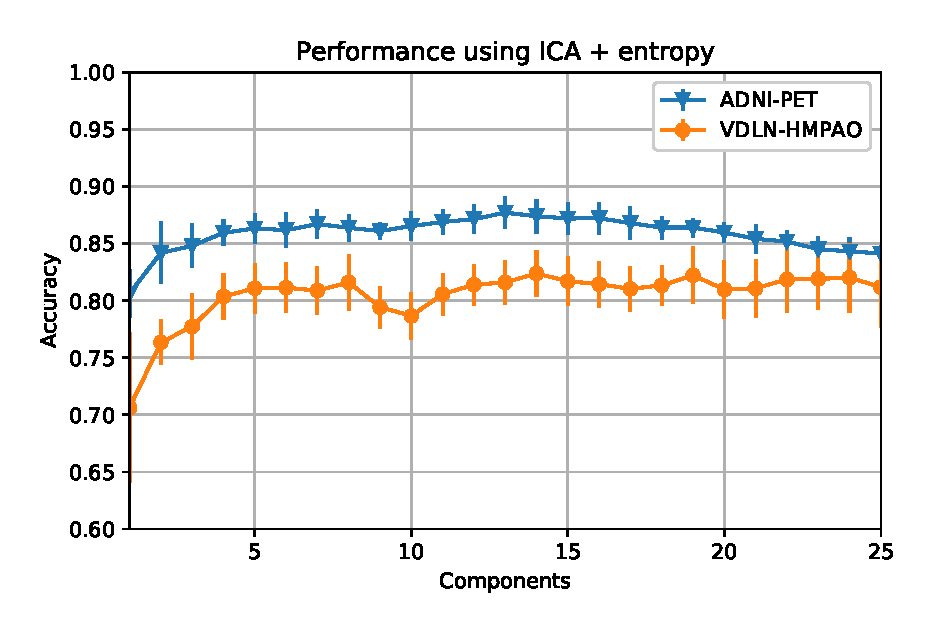
\includegraphics[width=0.49\linewidth]{Graphics/ch4/accuracyMeanSTD-ICA_vsK_entropy_AD.eps}\label{fig:AD-AV-ICA-ENTROPY-VSK}}
	
	\subfloat[]{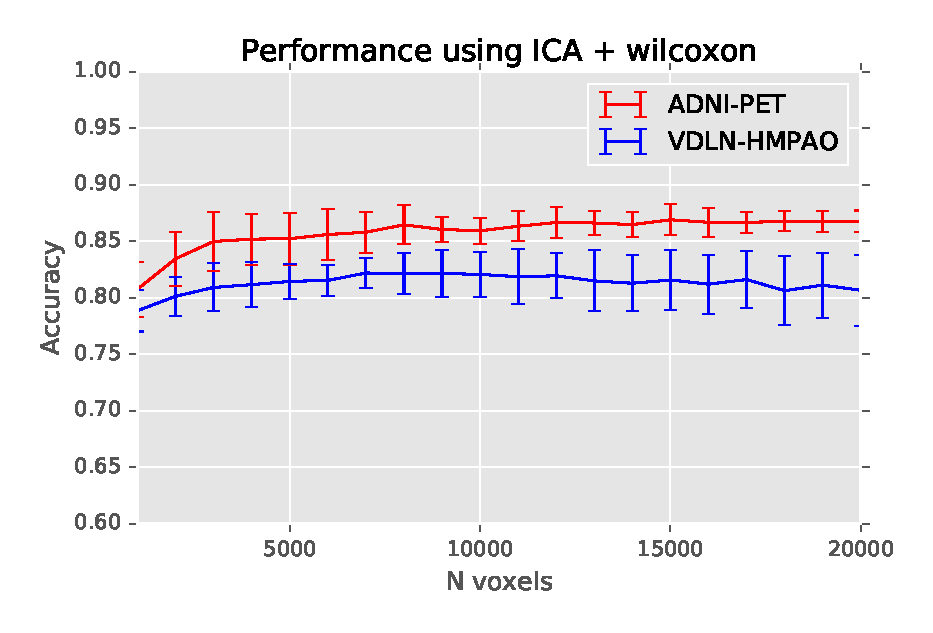
\includegraphics[width=0.49\linewidth]{Graphics/ch4/accuracyMeanSTD-ICA_vsN_wilcoxon_AD.eps}\label{fig:AD-AV-ICA-WILCOXON-VSN}}
	\subfloat[]{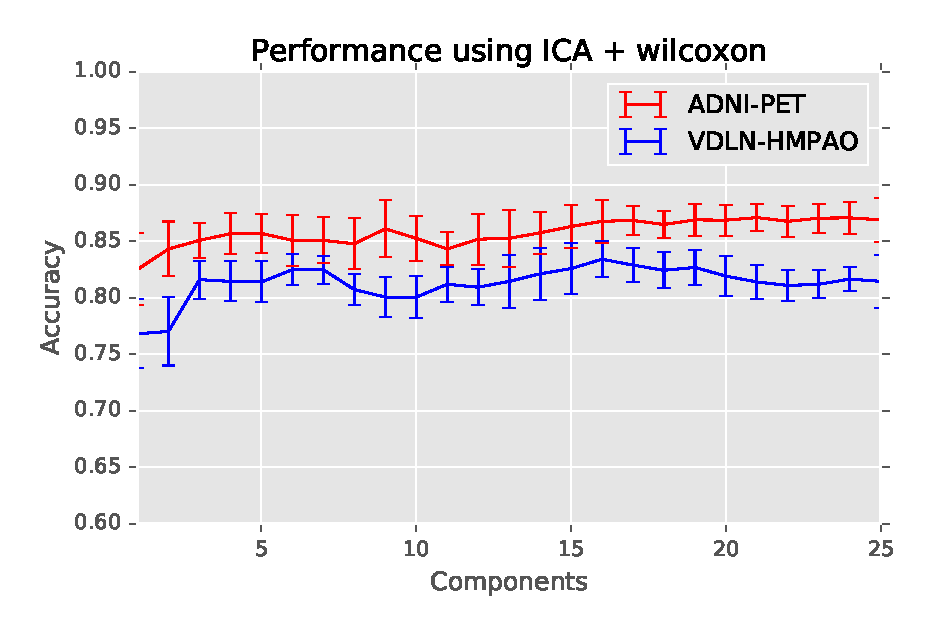
\includegraphics[width=0.49\linewidth]{Graphics/ch4/accuracyMeanSTD-ICA_vsK_wilcoxon_AD.eps}\label{fig:AD-AV-ICA-WILCOXON-VSK}}
	
	\caption[Average performance of the \acs{AD} datasets in \acs{ICA}.]{Average performance and standard deviation of the proposed system using the three \ac{AD} datasets, \ac{ICA} and the three feature selection criteria: $t$-test (\protect\subref{fig:AD-AV-ICA-TTEST-VSN} and \protect\subref{fig:AD-AV-ICA-TTEST-VSK}), relative entropy (\protect\subref{fig:AD-AV-ICA-ENTROPY-VSN} and \protect\subref{fig:AD-AV-ICA-ENTROPY-VSK}) and wilcoxon (\protect\subref{fig:AD-AV-ICA-WILCOXON-VSN} and \protect\subref{fig:AD-AV-ICA-WILCOXON-VSK}). } 
	\label{fig:accuracyMeanICA-AD}
\end{figure}

The case is similar to the one presented in section~\ref{sec:results_FA_AD}, where the performance slightly improves when increasing the number of selected voxels. The performance is again better when using the \adnipet{} dataset than with the \vdlnhmpao{}, although the behaviour is similar. 

The results change when varying the number of components. In this case, although good performance is obtained within the first 5 components in most cases, the model achieves similar performance in both datasets with components between 5 and 10, and then, the estimates diverge. In the \vdlnhmpao{}, the performance starts to decrease after this number of components, whereas when using the \adnipet{} dataset, the higher average performance is obtained with $c>15$, especially in the case of the $t$-test or the wilcoxon selection criteria). 

\subsubsection{At the Operation Point}
Now we focus on non-averaged values, the values for which our system is optimal: the operation point. In this scenario we see that the tendency is that all systems behave similarly. 

When increasing the number of selected voxels, we can see that there is always a tendency of slightly increase in both datasets and decomposition strategies, as can be seen in Figure~\ref{fig:accuracyOP-ADvsN}. For the \adnipet{} dataset, the maximum accuracies are obtained with a large number of voxels $f>15000$, however, in the case of \vdlnhmpao{}, we obtain similar performance with fewer voxels, $f<7000$ in all selection criteria. 

\begin{figure}
	\centering
	\subfloat[]{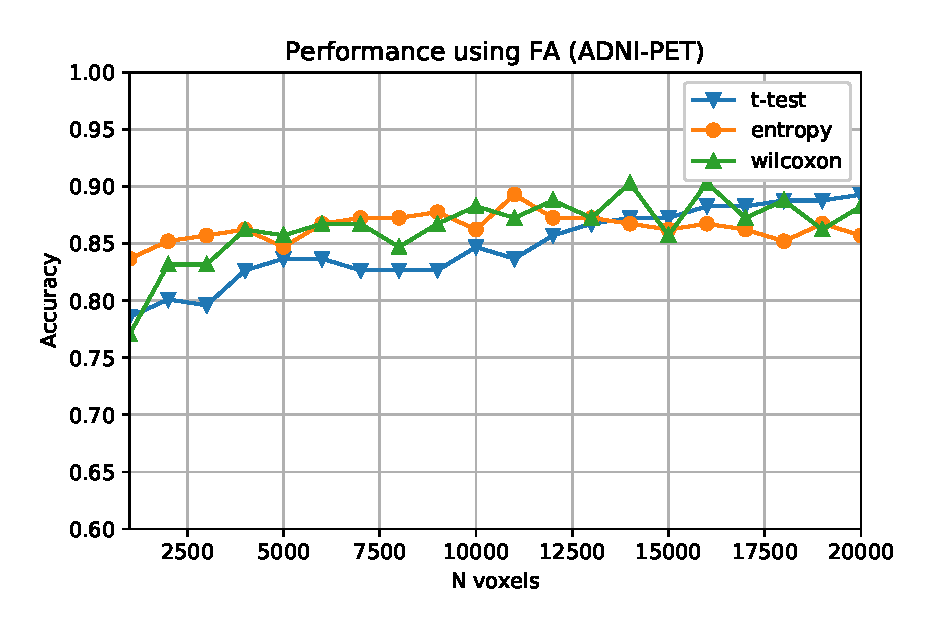
\includegraphics[width=0.49\linewidth]{Graphics/ch4/accuracyOP-FA_vsK_comparison_ADNI-PET.eps}\label{fig:ADNI-PET-FA-OP-VSN}}
	\subfloat[]{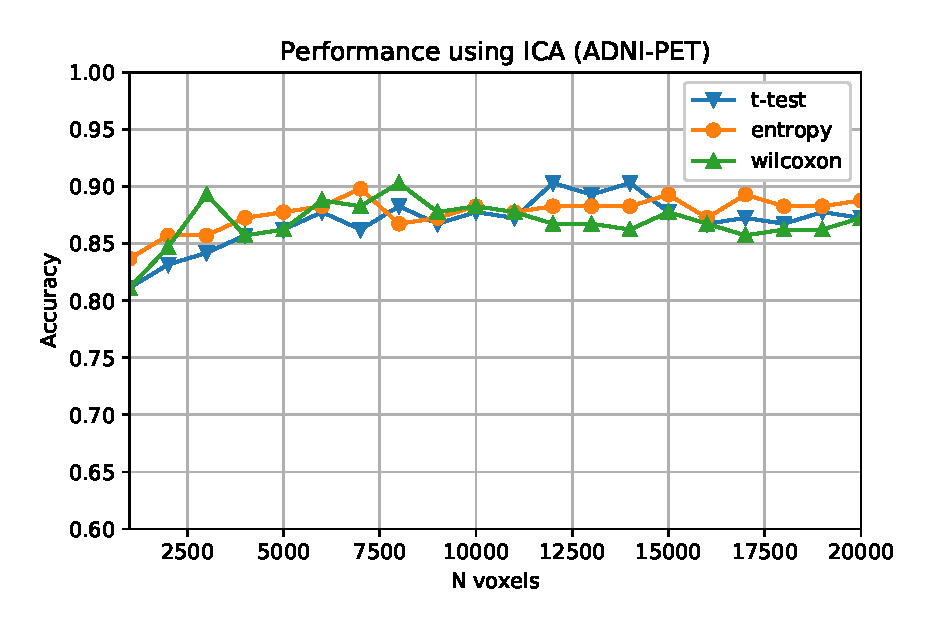
\includegraphics[width=0.49\linewidth]{Graphics/ch4/accuracyOP-ICA_vsK_comparison_ADNI-PET.eps}\label{fig:ADNI-PET-ICA-OP-VSN}}
	
	\subfloat[]{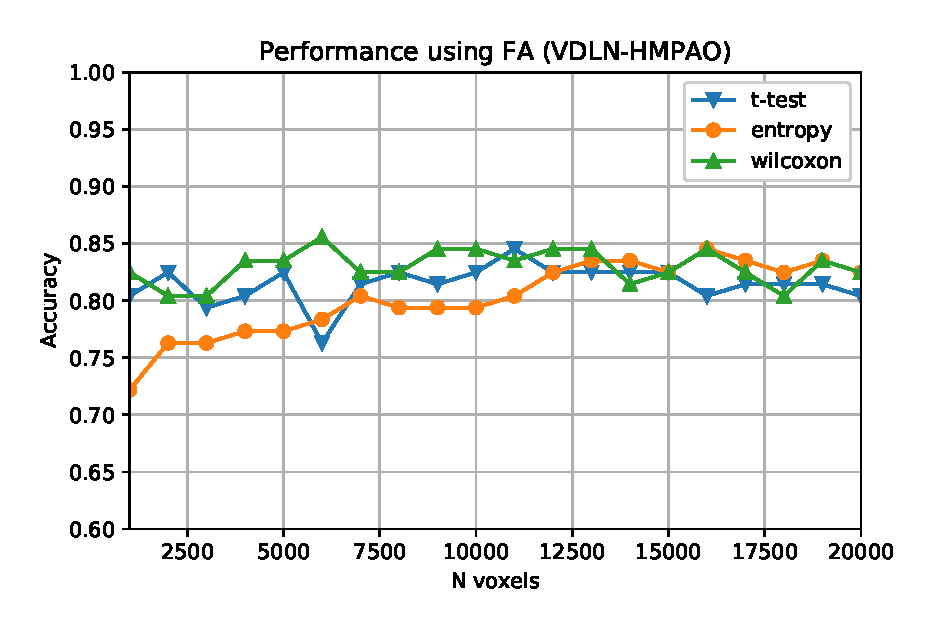
\includegraphics[width=0.49\linewidth]{Graphics/ch4/accuracyOP-FA_vsK_comparison_VDLN-HMPAO.eps}\label{fig:VDLN-HMPAO-FA-OP-VSN}}
	\subfloat[]{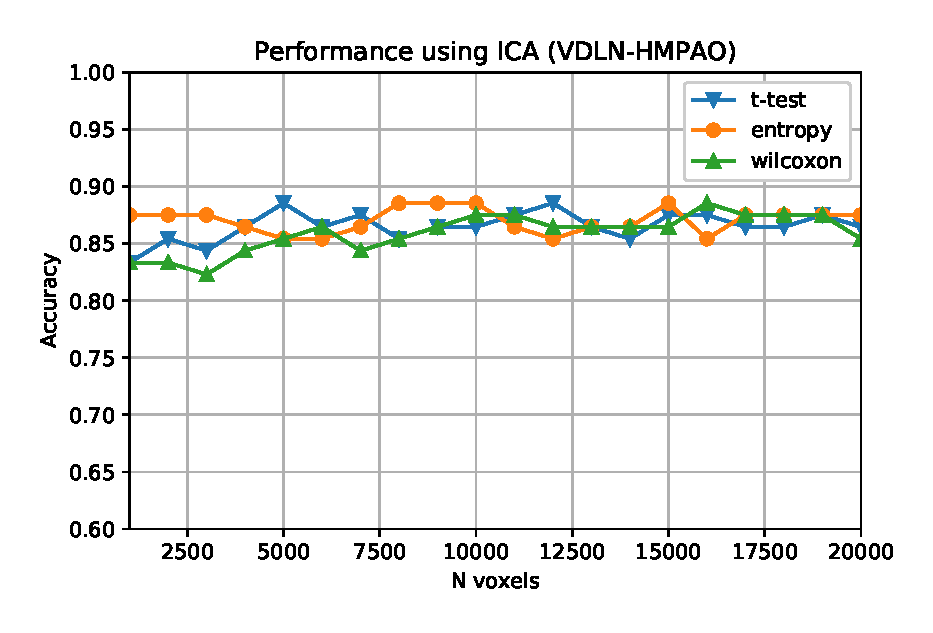
\includegraphics[width=0.49\linewidth]{Graphics/ch4/accuracyOP-ICA_vsK_comparison_VDLN-HMPAO.eps}\label{fig:VDLN-HMPAO-ICA-OP-VSN}}
	
	\caption[Performance at the operation point for the \acs{AD} datasets, over the number of selected voxels.]{Performance of the proposed system using the two \ac{AD} datasets: \adnipet{} and \vdlnhmpao{} at the operation point, and how they vary over the number of selected voxels. } 
	\label{fig:accuracyOP-ADvsN}
\end{figure}

Now we can focus on the performance variations over the number of components in Figure~\ref{fig:accuracyOP-AD}. The accuracy slightly varies almost in any case, and there is a steep increase in the performance within the first five components in both \ac{FA} and \ac{ICA}. 

\begin{figure}
	\centering
	\subfloat[]{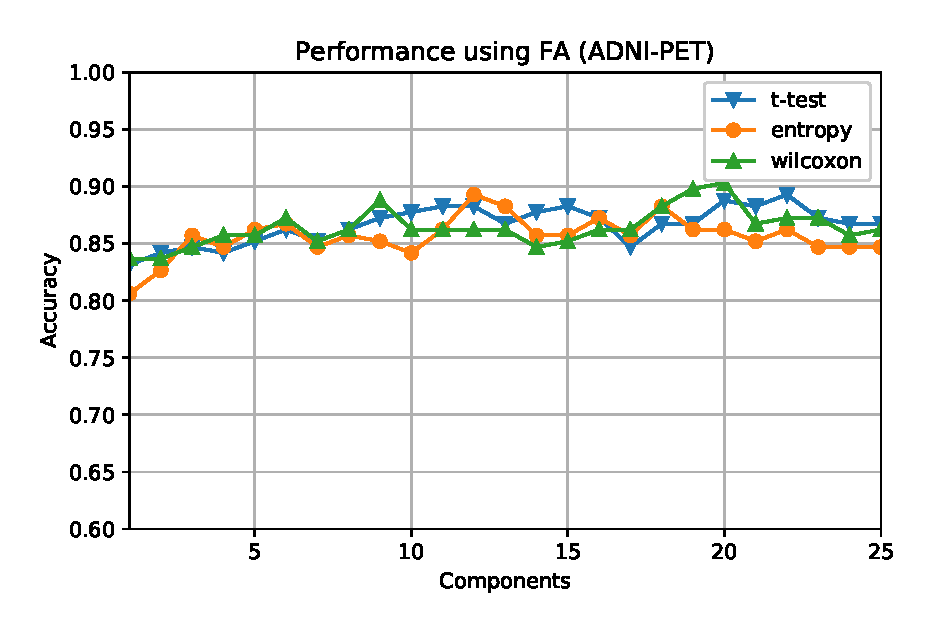
\includegraphics[width=0.49\linewidth]{Graphics/ch4/accuracyOP-FA_vsN_comparison_ADNI-PET.eps}\label{fig:ADNI-PET-FA-OP-VSK}}
	\subfloat[]{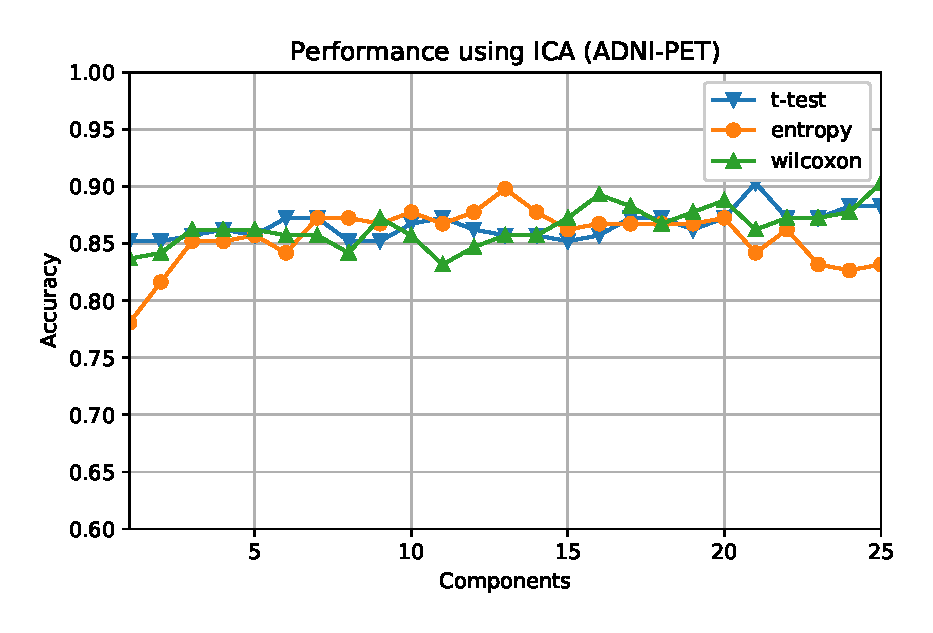
\includegraphics[width=0.49\linewidth]{Graphics/ch4/accuracyOP-ICA_vsN_comparison_ADNI-PET.eps}\label{fig:ADNI-PET-ICA-OP-VSK}}
	
	\subfloat[]{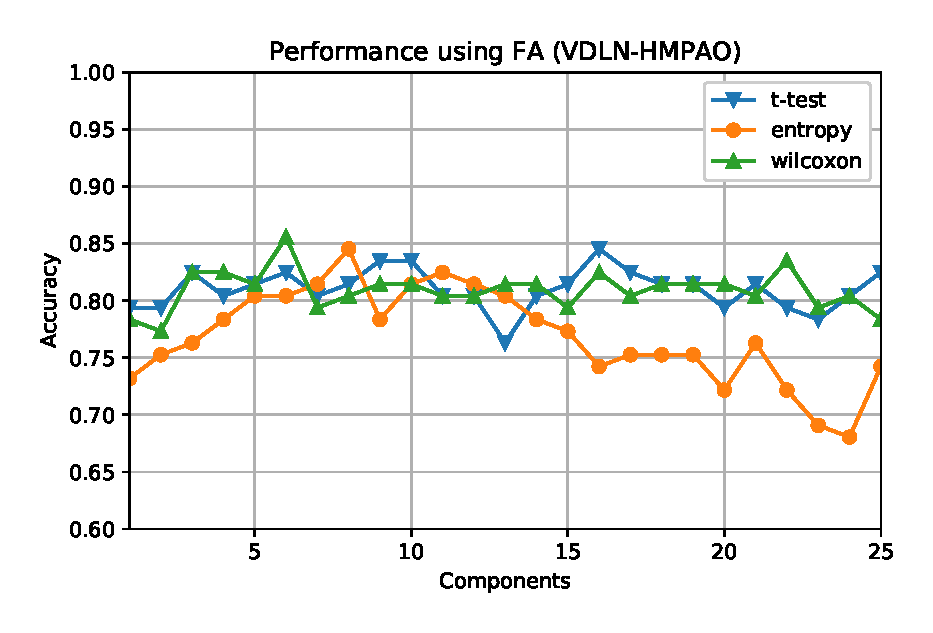
\includegraphics[width=0.49\linewidth]{Graphics/ch4/accuracyOP-FA_vsN_comparison_VDLN-HMPAO.eps}\label{fig:VDLN-HMPAO-FA-OP-VSK}}
	\subfloat[]{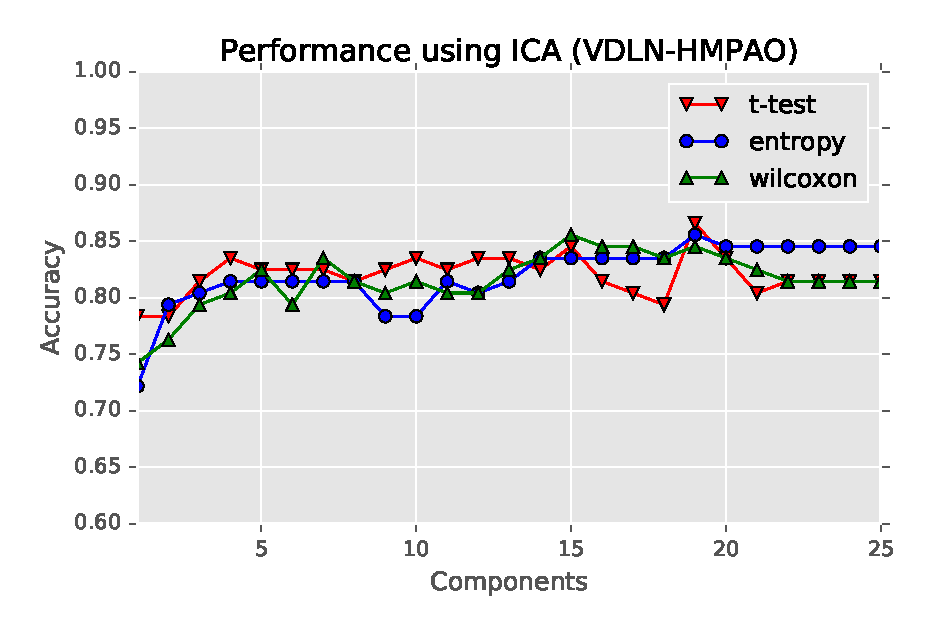
\includegraphics[width=0.49\linewidth]{Graphics/ch4/accuracyOP-ICA_vsN_comparison_VDLN-HMPAO.eps}\label{fig:VDLN-HMPAO-ICA-OP-VSK}}
	
	\caption[Performance at the operation point for the \acs{AD} datasets, over the number of components.]{Performance of the proposed system using the two \ac{AD} datasets: \adnipet{} and \vdlnhmpao{} at the operation point, and how they vary over the number of components used in the decomposition. } 
	\label{fig:accuracyOP-AD}
\end{figure}

A particular case is the combination of \ac{FA} and the relative entropy selection criteria applied to the \vdlnhmpao{} dataset. In this case there seems to be a trend to achieve a maximum performance at between 5 components. But with the \adnipet{} dataset, the performance keeps and achieves maximum accuracy with $c\approxeq 20$. 

In Table~\ref{tab:featureAD} we show the performance values obtained at the operation point for our different test combining decomposition algorithms and selection criteria, for the two datasets analysed in this section. It is obvious that both datasets obtain similar performance in almost every case, with values close to $0.9$. These values are compared to the baseline classification performance, quantified using \ac{VAF} \cite{Stoeckel04}. From this, we can see that the decomposition systems always perform better than the baseline, but this difference is especially large in the case of the \vdlnhmpao{} dataset, which contains very noisy images. 

\begin{table}
	\myfloatalign
	\begin{tabularx}{\linewidth}{Xllccc}
		\toprule
		\tableheadline{DB} & \tableheadline{Dec.} & \tableheadline{Criterion} & \tableheadline{Accuracy} & \tableheadline{Sensitivity} & \tableheadline{Specificity}\\
		\toprule
		\multirow{7}{1.7cm}{ADNI- PET} & \ac{VAF} & - & $0.882 \pm 0.064$ & $0.876 \pm 0.099$ & $0.890 \pm 0.097$ \\
		\cline{2-6}
		&  \multirow{3}{*}{\ac{FA}} & t-test & $ 0.893 \pm 0.074 $ & $ 0.886 \pm 0.119 $ & $ 0.901 \pm 0.101 $ \\
		&  & entropy & $ 0.893 \pm 0.074 $ & $ 0.894 \pm 0.092 $ & $ 0.891 \pm 0.088 $ \\
		&  & wilcoxon & $ 0.903 \pm 0.066 $ & $ 0.917 \pm 0.079 $ & $ 0.891 \pm 0.082 $ \\
		\cline{2-6}
		& \multirow{3}{*}{\ac{ICA}} & t-test & $ 0.903 \pm 0.071 $ & $ 0.893 \pm 0.100 $ & $ 0.910 \pm 0.107 $ \\
		&  & entropy & $ 0.898 \pm 0.059 $ & $ 0.917 \pm 0.088 $ & $ 0.881 \pm 0.084 $ \\
		&  & wilcoxon & $ 0.903 \pm 0.066 $ & $ 0.906 \pm 0.097 $ & $ 0.901 \pm 0.094 $ \\ \midrule
		\multirow{7}{1.7cm}{\vdlnhmpao{}} & \ac{VAF} & - & $0.802 \pm  0.074$ & $0.803 \pm 0.088$ & $0.805 \pm 0.145$ \\ 
		\cline{2-6}
		& \multirow{3}{*}{\ac{FA}} & t-test & $ 0.885 \pm 0.076 $ & $ 0.890 \pm 0.127 $ & $ 0.875 \pm 0.149 $ \\
		&  & entropy & $ 0.896 \pm 0.092 $ & $ 0.907 \pm 0.150 $ & $ 0.875 \pm 0.139 $ \\
		&  & wilcoxon & $ 0.885 \pm 0.076 $ & $ 0.923 \pm 0.130 $ & $ 0.825 \pm 0.154 $ \\
		\cline{2-6}
		& \multirow{3}{*}{\ac{ICA}} & t-test & $ 0.885 \pm 0.073 $ & $ 0.923 \pm 0.130 $ & $ 0.825 \pm 0.154 $ \\
		&  & entropy & $ 0.885 \pm 0.076 $ & $ 0.903 \pm 0.132 $ & $ 0.850 \pm 0.130 $ \\
		&  & wilcoxon & $ 0.885 \pm 0.076 $ & $ 0.907 \pm 0.130 $ & $ 0.850 \pm 0.152 $ \\
		\bottomrule
	\end{tabularx}
	\caption[Performance values for the Alzheimer's datasets]{Accuracy, sensitivity, specificity, and their standard deviation at the operation point for each method and its corresponding feature selection criterion, using two \protect\ac{AD} datasets. }
	\label{tab:featureAD}
\end{table}

Overall, all methods achieve similar values of accuracy, sensitivity and specificity. When analysing the \adnipet{} dataset, the wilcoxon selection criteria seems to outperform the rest especially with \ac{ICA}, with a higher accuracy and sensitivity. On the other hand, with the \vdlnhmpao{} dataset, either the $t$-test or the wilcoxon achieves higher sensitivity, but there is no difference in accuracy when decomposing with the \ac{ICA} algorithm. When using \ac{FA} decomposition, the relative entropy seems to perform better. In general, there seems to be little difference among methods, and a curious relationship between the relative entropy selection and the \vdlnhmpao{} dataset that we will discuss later. 

\FloatBarrier

\subsection{Parkinson's Disease}
Now we will look at how the proposed \ac{CAD} system behaves when applied to the three DaTSCAN datasets: \vdlndat{}, \vdlvdat{} and \ppmidat{}. For this experiment we will use a maximum of $1500$ selected voxels and $25$ components, and images that have been previously intensity normalized using the integral normalization algorithm (see section~\ref{sec:intensityPrep}). 

\subsubsection{Factor Analysis}
Firstly, we will explore the average behaviour of the system that uses \ac{FA} as a decomposition technique. For this purpose, as in previous sections, Figure~\ref{fig:accuracyMeanFA-PKS} shows how the average performance varies when varying the number of voxels selected and the number of components extracted. 

\begin{figure}
	\centering
	\subfloat[]{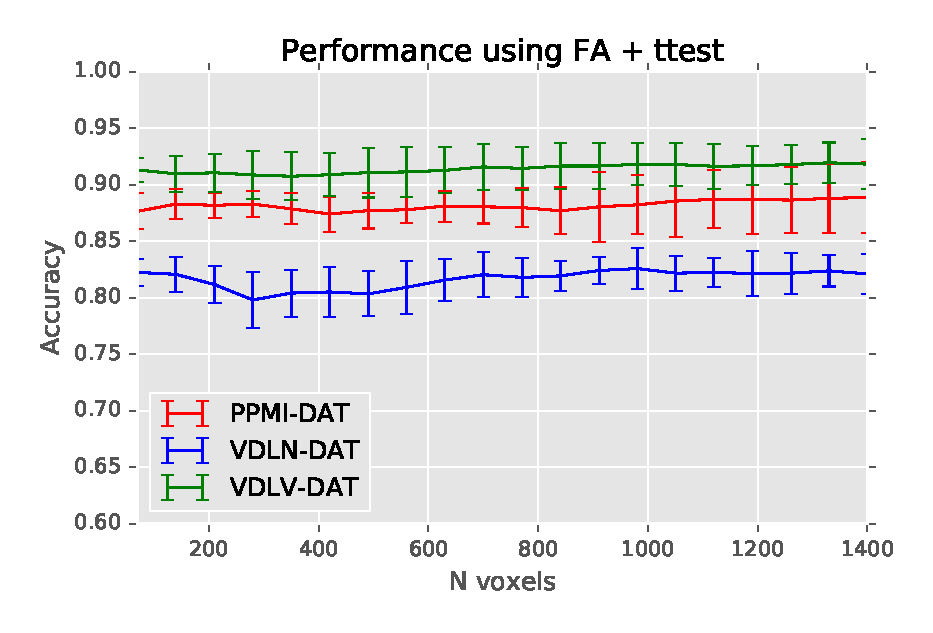
\includegraphics[width=0.49\linewidth]{Graphics/ch4/accuracyMeanSTD-FA_vsN_ttest_PKS.eps}\label{fig:PKS-AV-FA-TTEST-VSN}}
	\subfloat[]{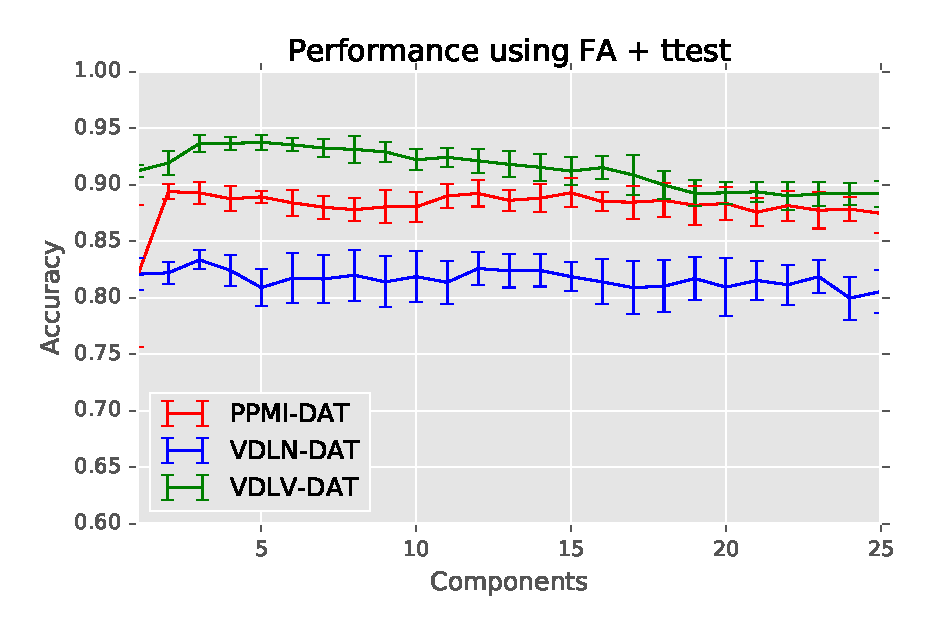
\includegraphics[width=0.49\linewidth]{Graphics/ch4/accuracyMeanSTD-FA_vsK_ttest_PKS.eps}\label{fig:PKS-AV-FA-TTEST-VSK}}
	
	\subfloat[]{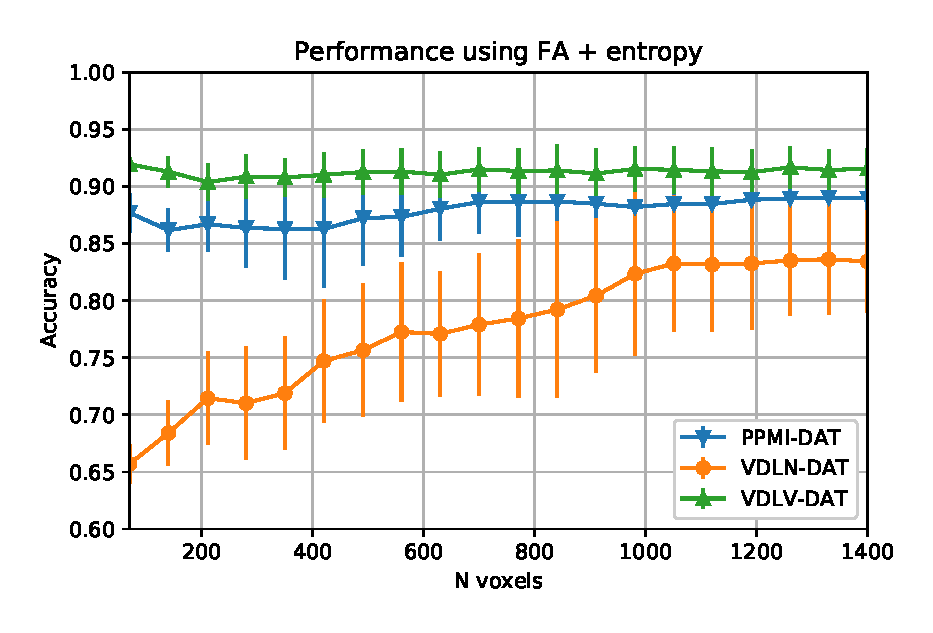
\includegraphics[width=0.49\linewidth]{Graphics/ch4/accuracyMeanSTD-FA_vsN_entropy_PKS.eps}\label{fig:PKS-AV-FA-ENTROPY-VSN}}
	\subfloat[]{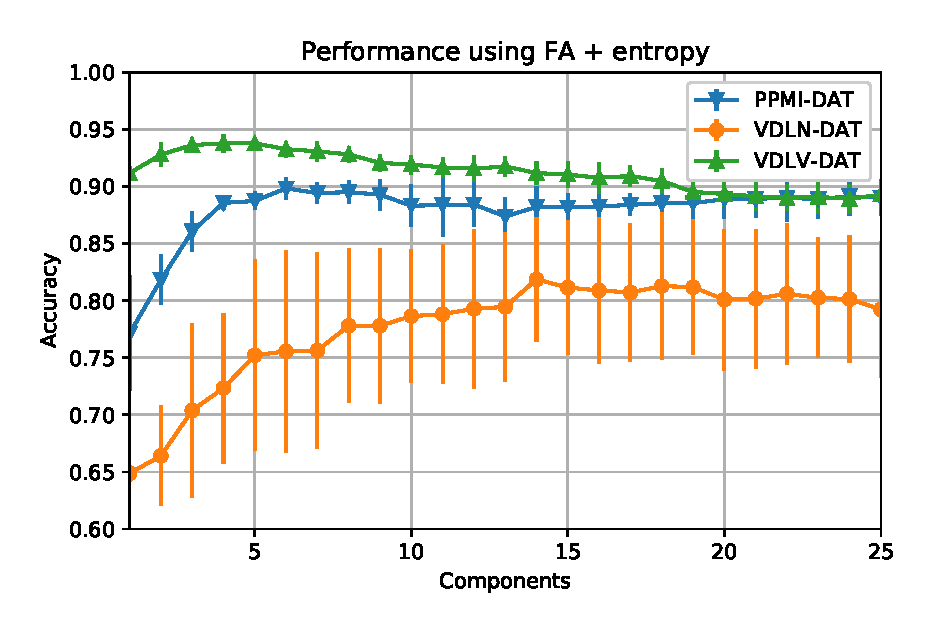
\includegraphics[width=0.49\linewidth]{Graphics/ch4/accuracyMeanSTD-FA_vsK_entropy_PKS.eps}\label{fig:PKS-AV-FA-ENTROPY-VSK}}
	
	\subfloat[]{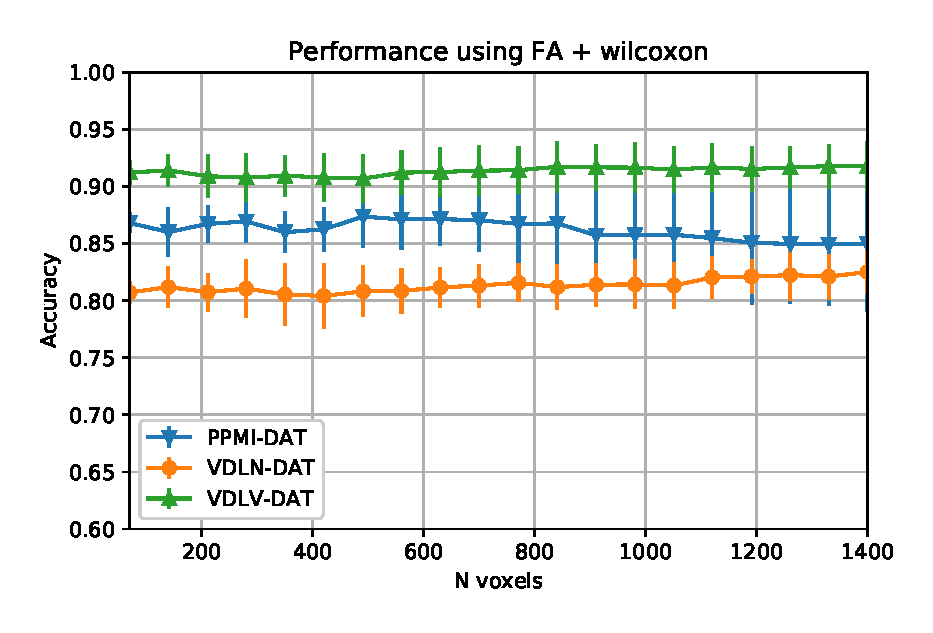
\includegraphics[width=0.49\linewidth]{Graphics/ch4/accuracyMeanSTD-FA_vsN_wilcoxon_PKS.eps}\label{fig:PKS-AV-FA-WILCOXON-VSN}}
	\subfloat[]{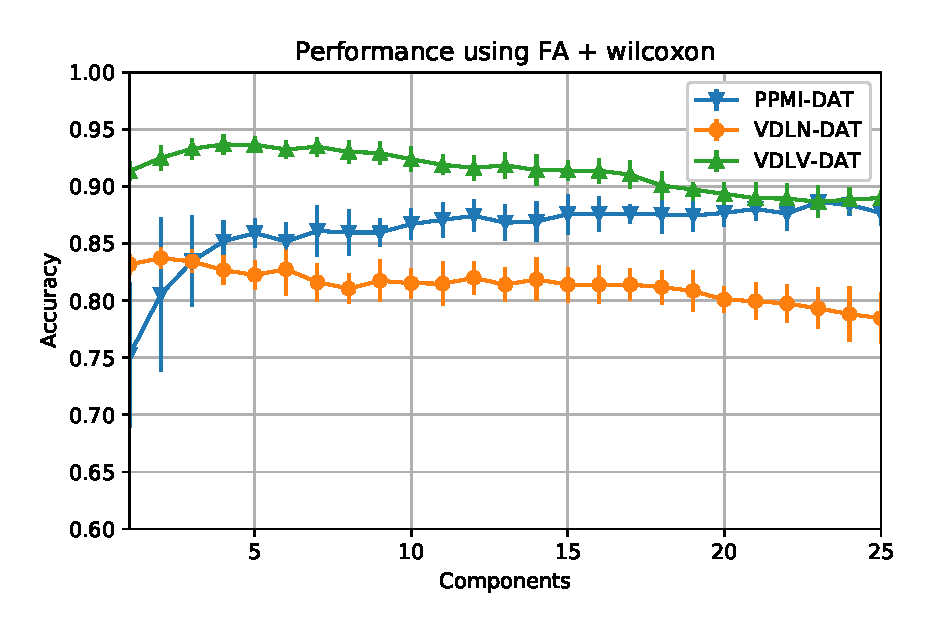
\includegraphics[width=0.49\linewidth]{Graphics/ch4/accuracyMeanSTD-FA_vsK_wilcoxon_PKS.eps}\label{fig:PKS-AV-FA-WILCOXON-VSK}}
	
	\caption[Average performance of the \acs{PKS} datasets in \acs{FA}.]{Average performance and standard deviation of the proposed system using the three \ac{PKS} datasets, \ac{FA} and the three feature selection criteria: $t$-test (\protect\subref{fig:PKS-AV-FA-TTEST-VSN} and \protect\subref{fig:PKS-AV-FA-TTEST-VSK}), relative entropy (\protect\subref{fig:PKS-AV-FA-ENTROPY-VSN} and \protect\subref{fig:PKS-AV-FA-ENTROPY-VSK}) and wilcoxon (\protect\subref{fig:PKS-AV-FA-WILCOXON-VSN} and \protect\subref{fig:PKS-AV-FA-WILCOXON-VSK}). } 
	\label{fig:accuracyMeanFA-PKS}
\end{figure}

In this case there is a clear difference between datasets, since some of them are more complex than others, usually due to a typical acquisition procedure in DaTSCAN. In the \vdlndat{}, the images were often composed only of a few cuts around the striatum, whereas in PPMI and \vdlvdat{} this rarely happens. That would explain the average outperformance of these two datasets over the \vdlndat{} in almost all cases. 

Their behaviours are consistent. Usually, there is no variation with the number of voxel selected (except in the obvious case of the \vdlndat{} dataset and the relative entropy selection criterion). However, there are repeated trends regarding the number of components or factors used in the computation. We can see that the performance increases in the first components, and once we have achieve a decent number (between 4 and 6), the performance starts to decrease. This could mean that the decomposition in more than 5 or 6 components only introduces noise and leads to a wrong decomposition. 

Again, this behaviour is consistent with the \vdlndat{} dataset, except for one case. It does seem that the interaction between the \vdlndat{} dataset and the relative entropy selection criterion leads to a wrong model. We will explore this question later, in the discussion. 

\subsubsection{Independent Component Analysis}
Regarding the application of the \ac{ICA} decomposition model to the DaTSCAN datasets. In Figure~\ref{fig:accuracyMeanICA-PKS} we present the average accuracy achieved by this model using three different selection criteria and the three \ac{PKS} datasets. 

\begin{figure}
	\subfloat[]{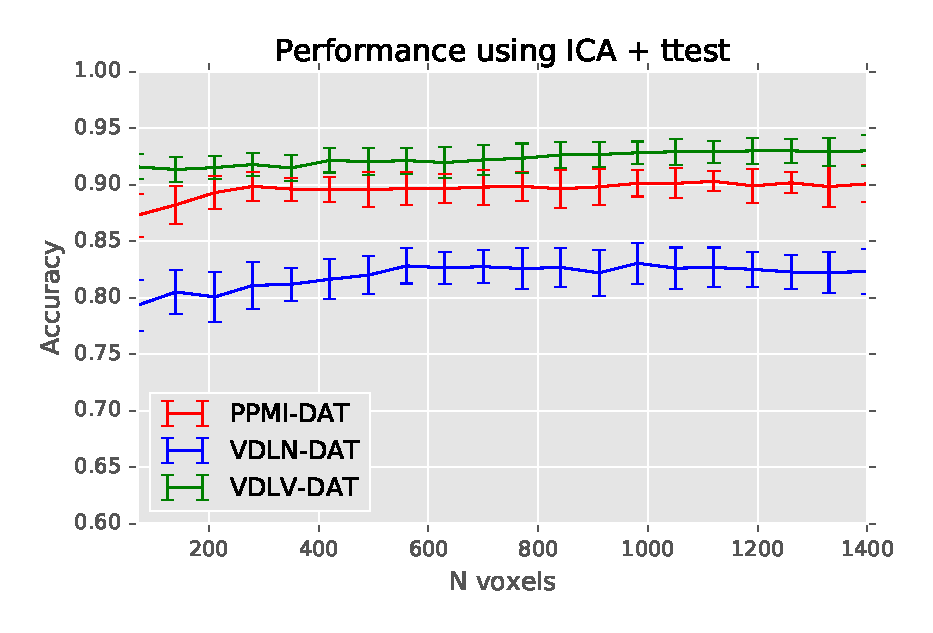
\includegraphics[width=0.49\linewidth]{Graphics/ch4/accuracyMeanSTD-ICA_vsN_ttest_PKS.eps}\label{fig:PKS-AV-ICA-TTEST-VSN}}
	\subfloat[]{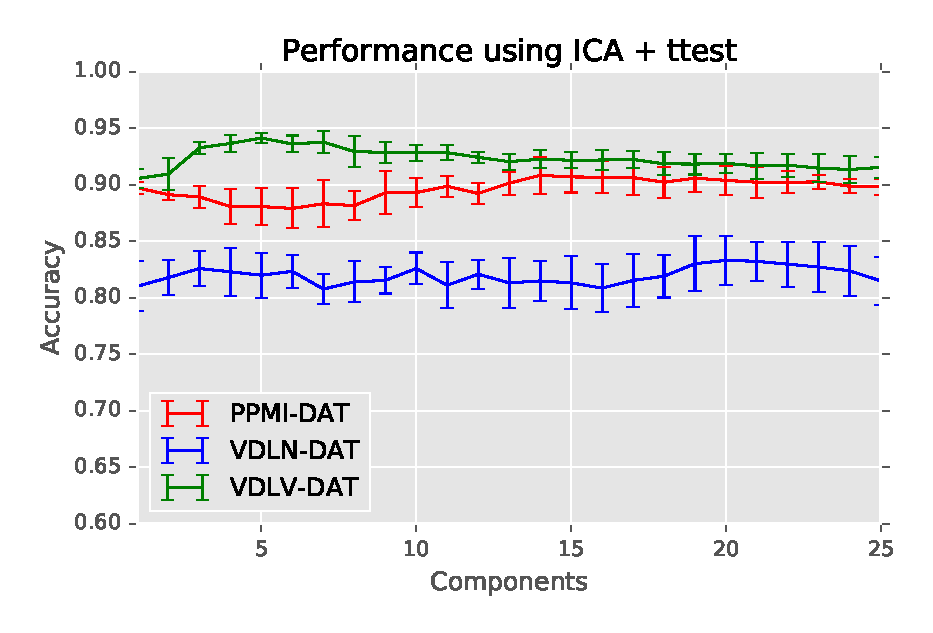
\includegraphics[width=0.49\linewidth]{Graphics/ch4/accuracyMeanSTD-ICA_vsK_ttest_PKS.eps}\label{fig:PKS-AV-ICA-TTEST-VSK}}
	
	\subfloat[]{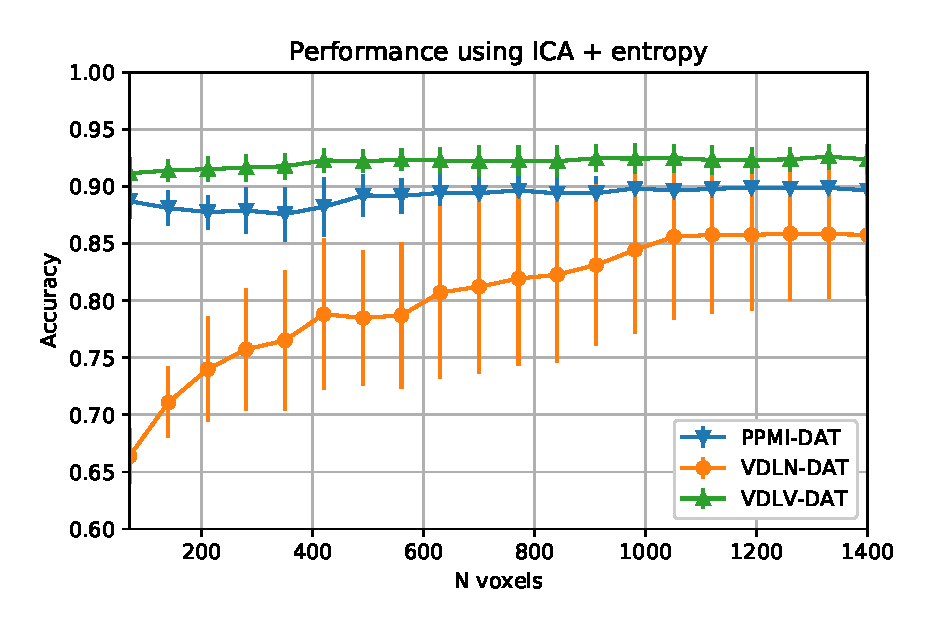
\includegraphics[width=0.49\linewidth]{Graphics/ch4/accuracyMeanSTD-ICA_vsN_entropy_PKS.eps}\label{fig:PKS-AV-ICA-ENTROPY-VSN}}
	\subfloat[]{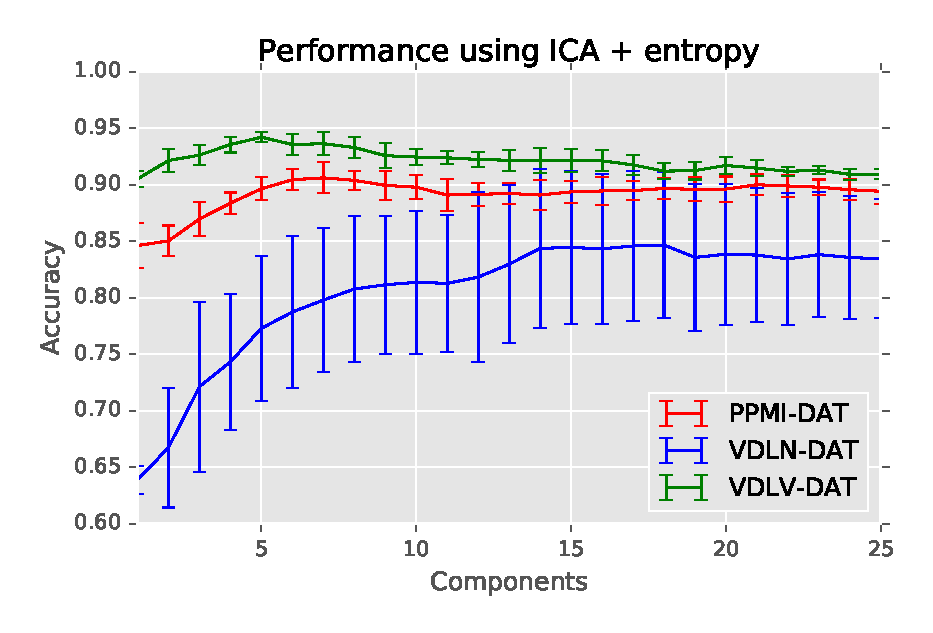
\includegraphics[width=0.49\linewidth]{Graphics/ch4/accuracyMeanSTD-ICA_vsK_entropy_PKS.eps}\label{fig:PKS-AV-ICA-ENTROPY-VSK}}
	
	\subfloat[]{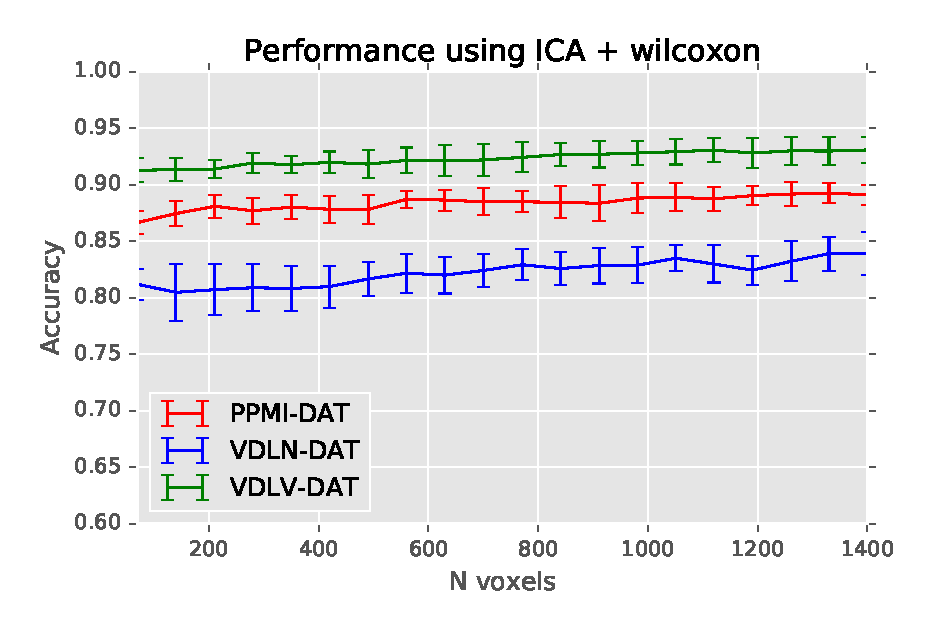
\includegraphics[width=0.49\linewidth]{Graphics/ch4/accuracyMeanSTD-ICA_vsN_wilcoxon_PKS.eps}\label{fig:PKS-AV-ICA-WILCOXON-VSN}}
	\subfloat[]{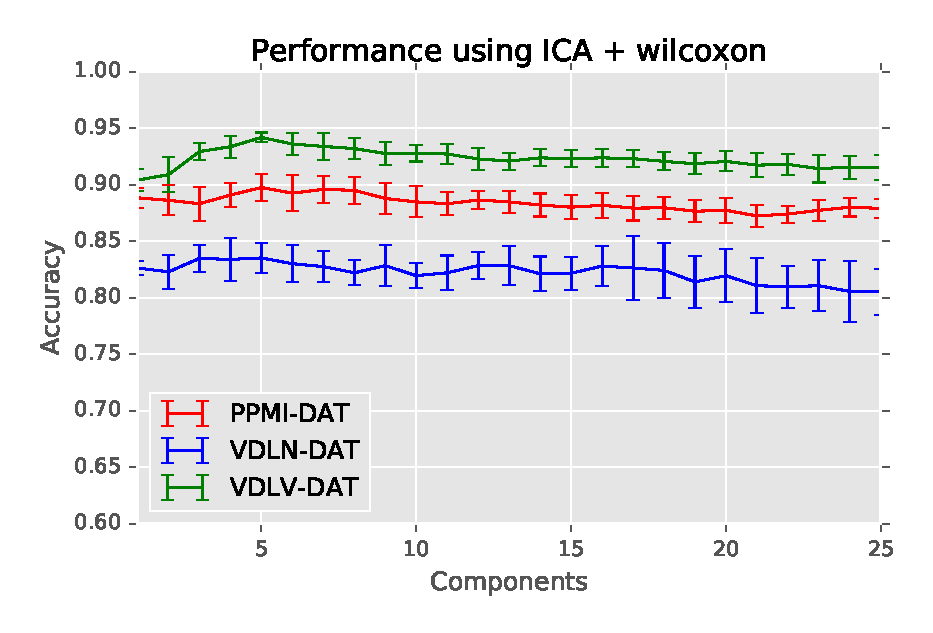
\includegraphics[width=0.49\linewidth]{Graphics/ch4/accuracyMeanSTD-ICA_vsK_wilcoxon_PKS.eps}\label{fig:PKS-AV-ICA-WILCOXON-VSK}}
	
	\caption[Average performance of the \acs{PKS} datasets in \acs{ICA}.]{Average performance and standard deviation of the proposed system using the three \ac{PKS} datasets, \ac{ICA} and the three feature selection criteria: $t$-test (\protect\subref{fig:PKS-AV-ICA-TTEST-VSN} and \protect\subref{fig:PKS-AV-ICA-TTEST-VSK}), relative entropy (\protect\subref{fig:PKS-AV-ICA-ENTROPY-VSN} and \protect\subref{fig:PKS-AV-ICA-ENTROPY-VSK}) and wilcoxon (\protect\subref{fig:PKS-AV-ICA-WILCOXON-VSN} and \protect\subref{fig:PKS-AV-ICA-WILCOXON-VSK}). } 
	\label{fig:accuracyMeanICA-PKS}
\end{figure}

In average, \ppmidat{} and \vdlvdat{} achieve similar performance, while \vdlndat{} generally achieves much poorer results. However, the behaviour of the system when varying the number of voxels or number of components is similar in all three datasets. The tendency is that accuracy does not significantly vary when increasing the number of voxels (except in the case of the relative entropy and \vdlndat{}). In contrast, when varying the number of components, we observe that the maximum performance is achieved in the first components, typically between 5 and 10. 

\subsubsection{At the Operation Point}
Let us now have a look at the behaviour of this system at the operation point, using the parameters $c$ and $f$ for which our system is optimal. When varying the number of voxels selected, we obtain the graphs presented at Figure~\ref{fig:accuracyOP-PKSvsN}. 

\begin{figure}
	\subfloat[]{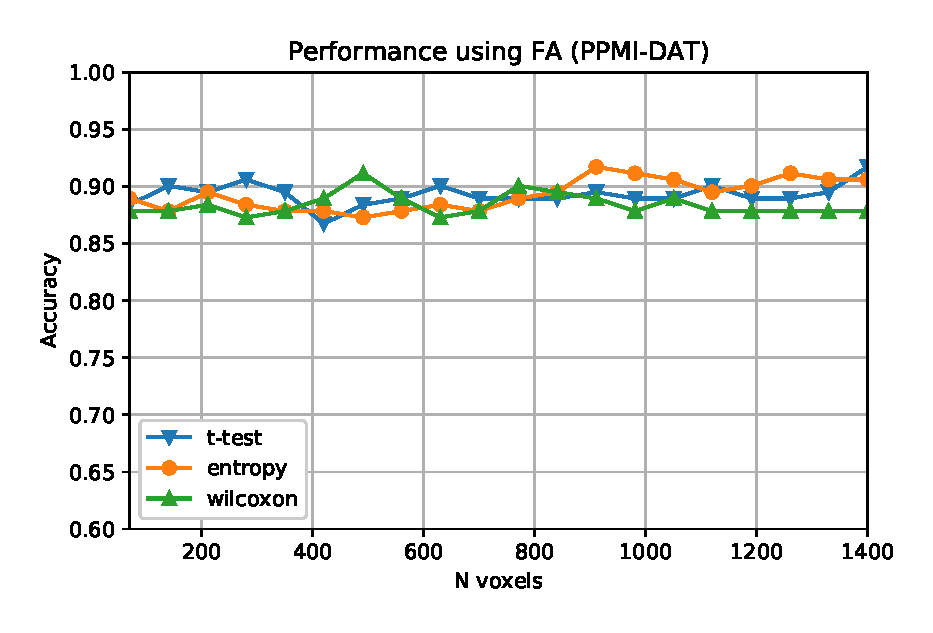
\includegraphics[width=0.49\linewidth]{Graphics/ch4/accuracyOP-FA_vsK_comparison_PPMI-DAT.eps}\label{fig:PPMI-DAT-FA-OP-vsN}}
	\subfloat[]{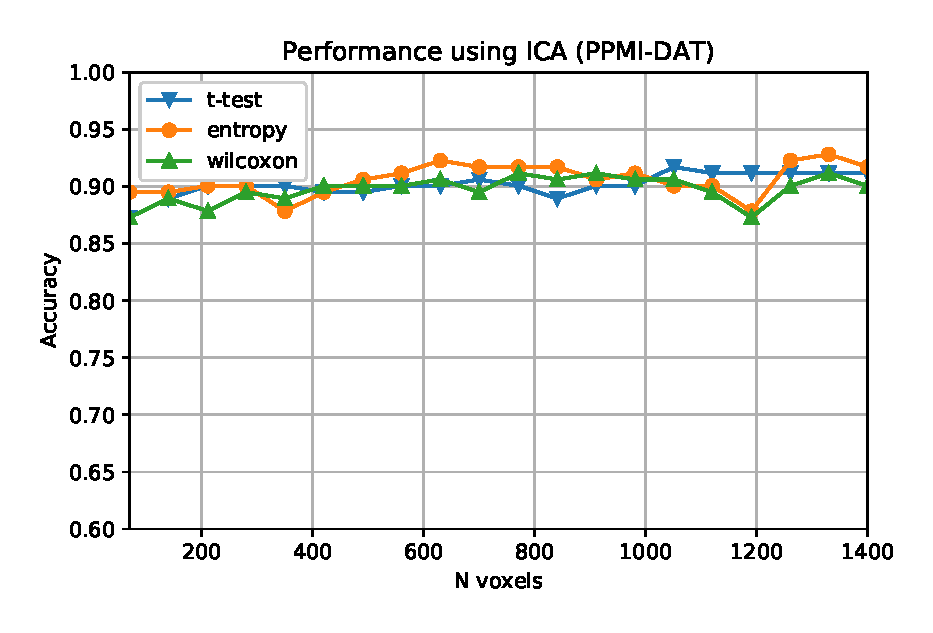
\includegraphics[width=0.49\linewidth]{Graphics/ch4/accuracyOP-ICA_vsK_comparison_PPMI-DAT.eps}\label{fig:PPMI-DAT-ICA-OP-vsN}}
	
	\subfloat[]{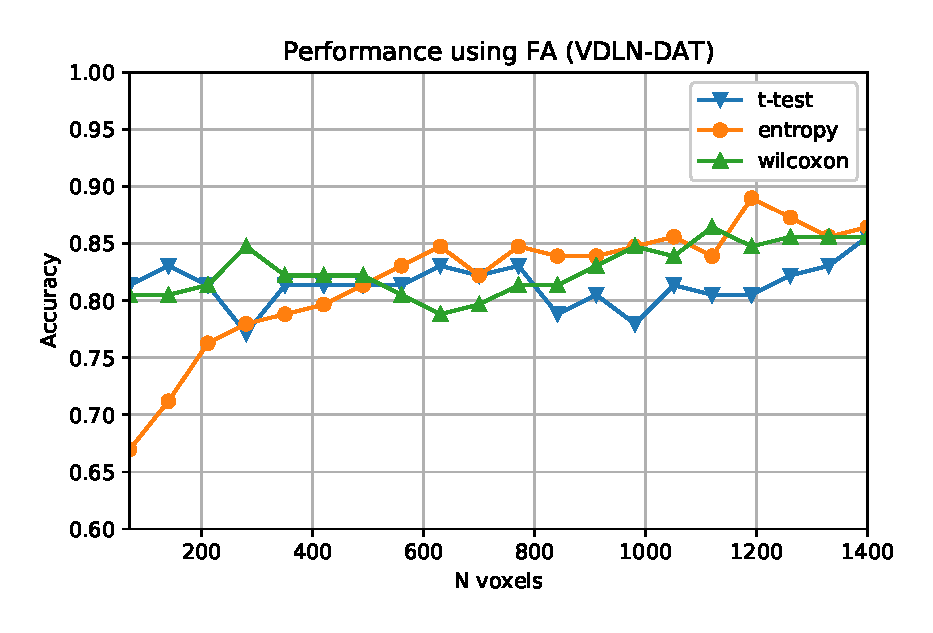
\includegraphics[width=0.49\linewidth]{Graphics/ch4/accuracyOP-FA_vsK_comparison_VDLN-DAT.eps}\label{fig:VDLN-DAT-FA-OP-vsN}}
	\subfloat[]{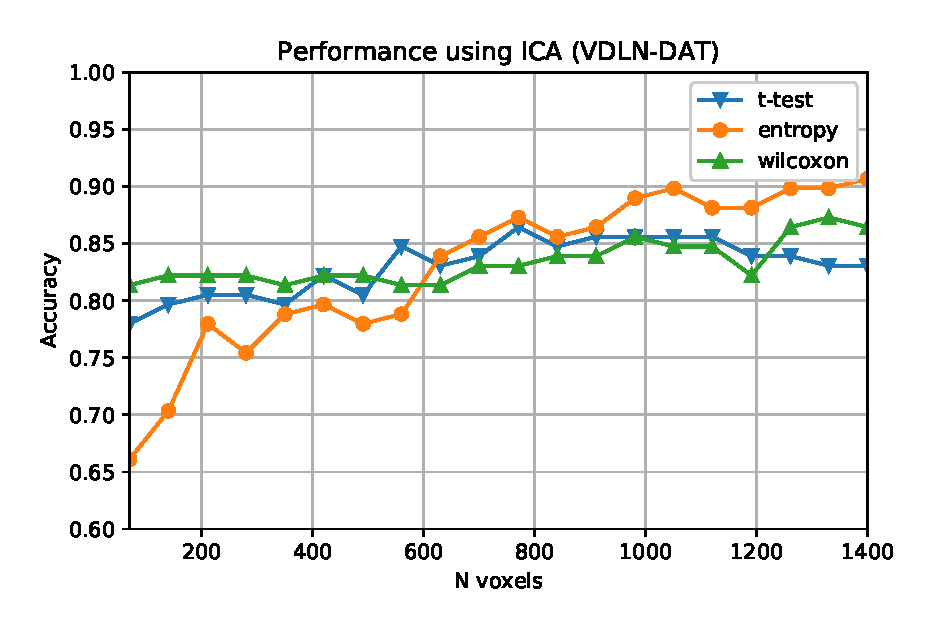
\includegraphics[width=0.49\linewidth]{Graphics/ch4/accuracyOP-ICA_vsK_comparison_VDLN-DAT.eps}\label{fig:VDLN-DAT-ICA-OP-vsN}}
	
	\subfloat[]{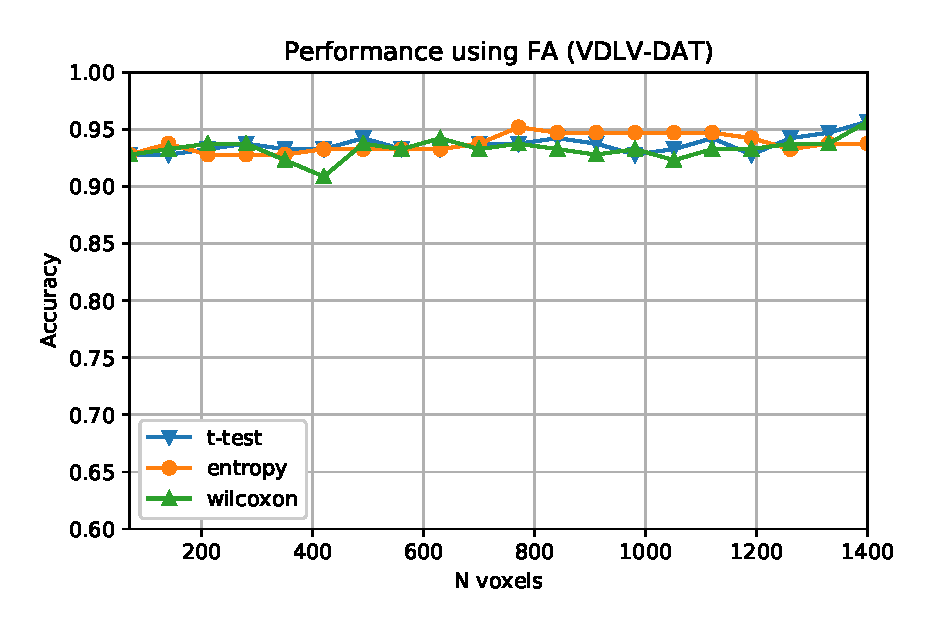
\includegraphics[width=0.49\linewidth]{Graphics/ch4/accuracyOP-FA_vsK_comparison_VDLV-DAT.eps}\label{fig:VDLV-DAT-FA-OP-vsN}}
	\subfloat[]{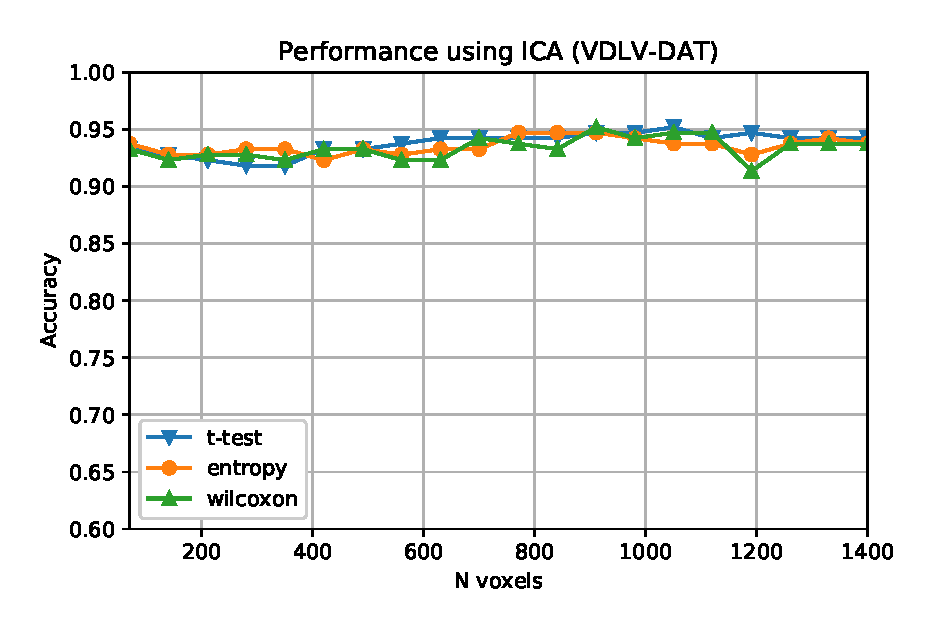
\includegraphics[width=0.49\linewidth]{Graphics/ch4/accuracyOP-ICA_vsK_comparison_VDLV-DAT.eps}\label{fig:VDLV-DAT-ICA-OP-vsN}}
	
	\caption[Performance at the operation point for the \acs{PKS} datasets, over the number of selected voxels.]{Performance of the proposed system using the two \ac{PKS} datasets: \ppmidat{}, \vdlndat{} and \vdlvdat{} at the operation point, and how they vary over the number of selected voxels. } 
	\label{fig:accuracyOP-PKSvsN}
\end{figure}

In this case, we obtain again that our system maintains approximately the same performance regardless of the number of voxels selected when tested on both the \ppmidat{} and the \vdlvdat{} datasets. In contrast, the performance increases when increasing the number of selected voxels when testing the \vdlndat{} dataset, especially when using the relative entropy criterion. This latter dataset also obtains less performance, whereas the \vdlvdat{} achieves the best. 

As for the changes in performance when varying the number of components, the results for both \ac{FA} and \ac{ICA} based systems are shown in Figure~\ref{fig:accuracyOP-PKS}. 

\begin{figure}
	\subfloat[]{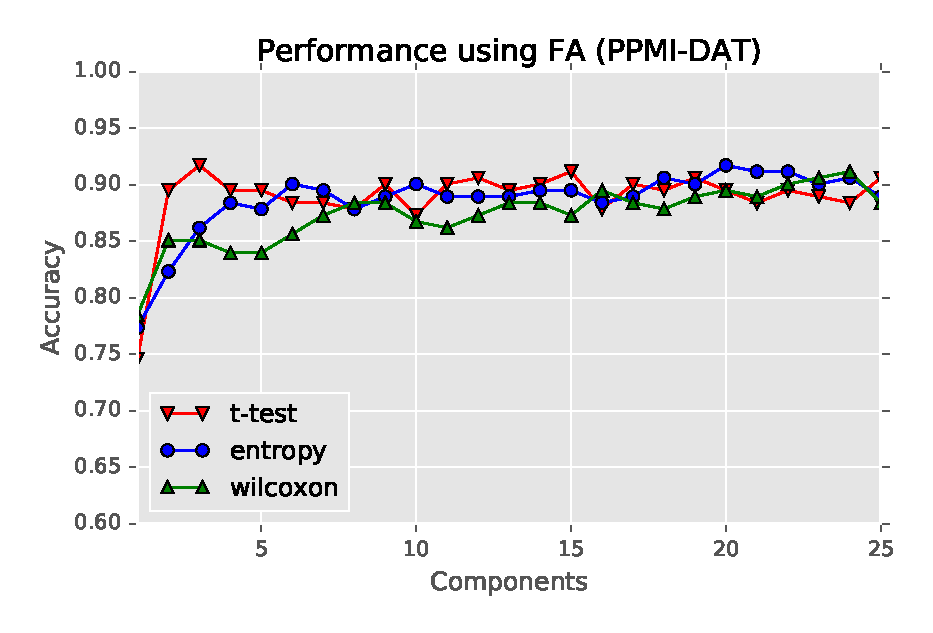
\includegraphics[width=0.49\linewidth]{Graphics/ch4/accuracyOP-FA_vsN_comparison_PPMI-DAT.eps}\label{fig:PPMI-DAT-FA-OP}}
	\subfloat[]{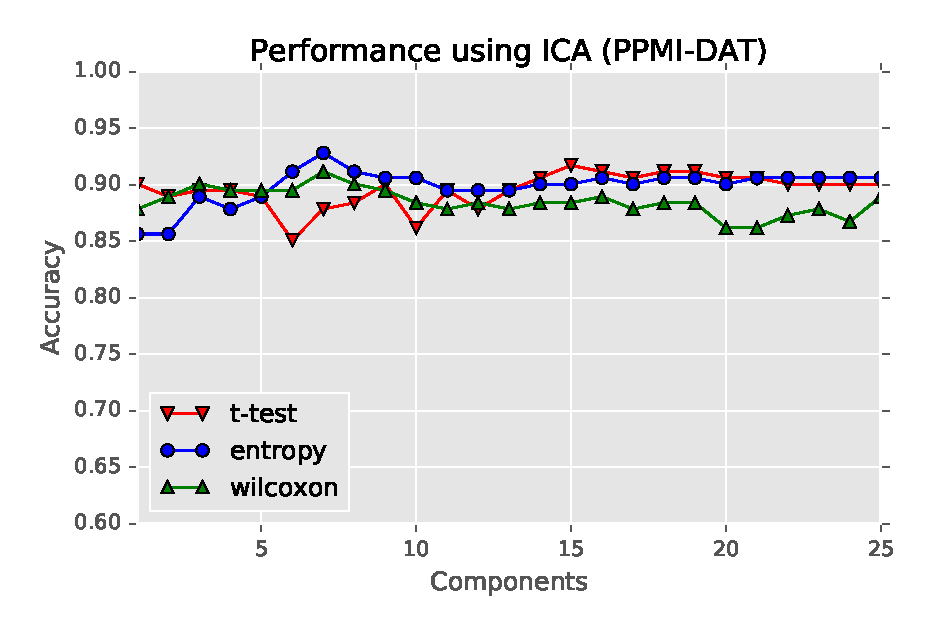
\includegraphics[width=0.49\linewidth]{Graphics/ch4/accuracyOP-ICA_vsN_comparison_PPMI-DAT.eps}\label{fig:PPMI-DAT-ICA-OP}}
	
	\subfloat[]{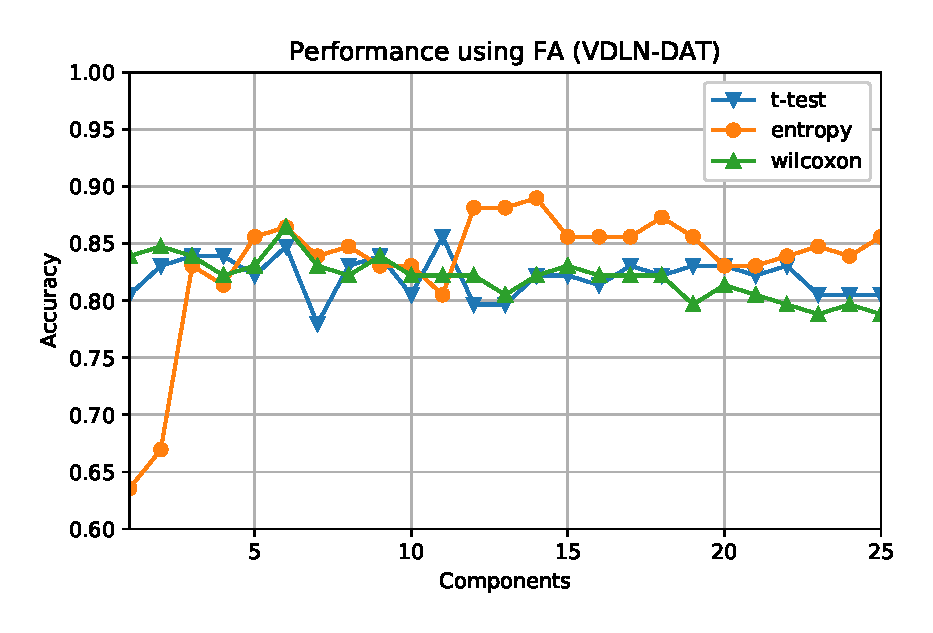
\includegraphics[width=0.49\linewidth]{Graphics/ch4/accuracyOP-FA_vsN_comparison_VDLN-DAT.eps}\label{fig:VDLN-DAT-FA-OP}}
	\subfloat[]{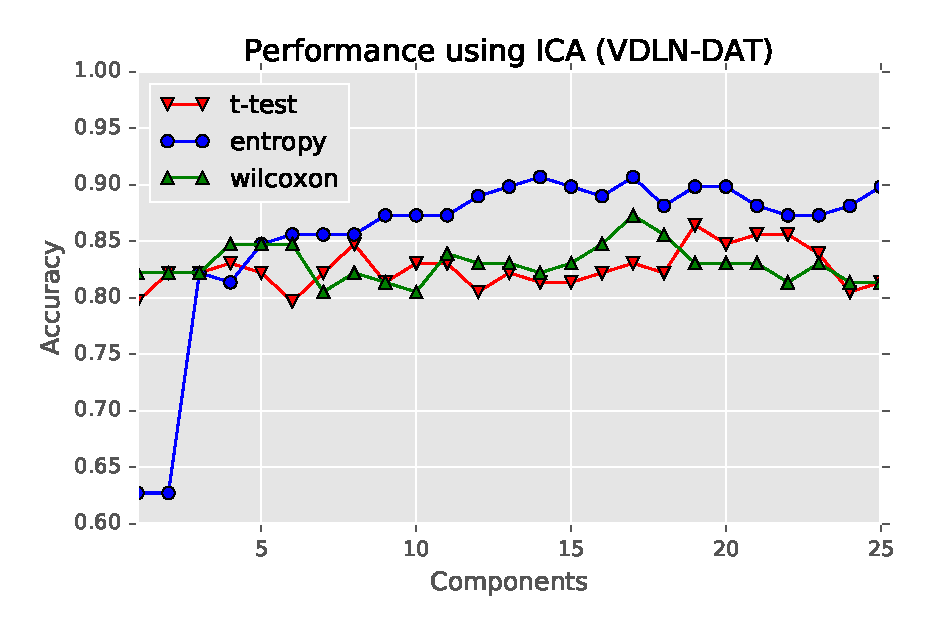
\includegraphics[width=0.49\linewidth]{Graphics/ch4/accuracyOP-ICA_vsN_comparison_VDLN-DAT.eps}\label{fig:VDLN-DAT-ICA-OP}}
	
	\subfloat[]{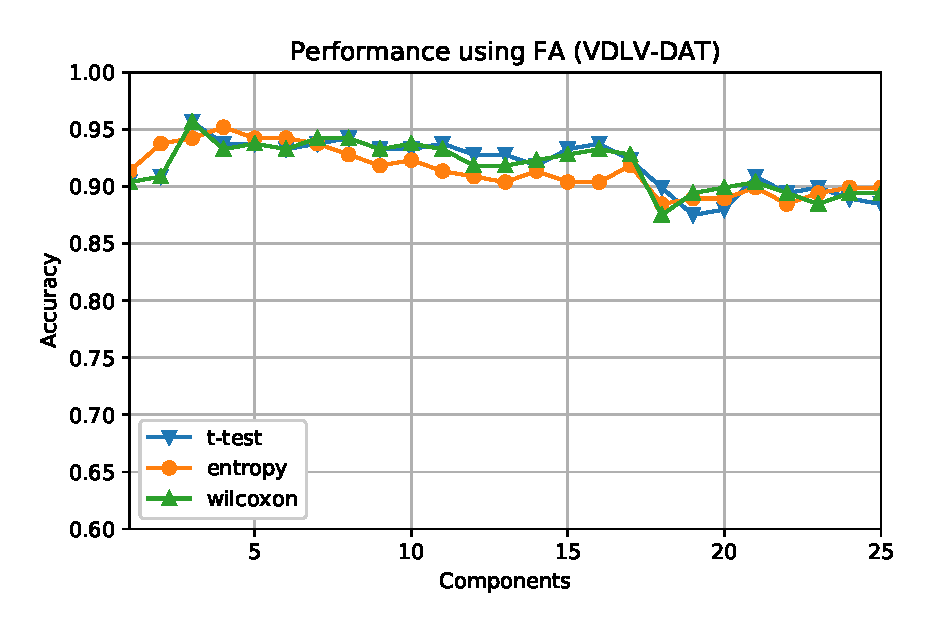
\includegraphics[width=0.49\linewidth]{Graphics/ch4/accuracyOP-FA_vsN_comparison_VDLV-DAT.eps}\label{fig:VDLV-DAT-FA-OP}}
	\subfloat[]{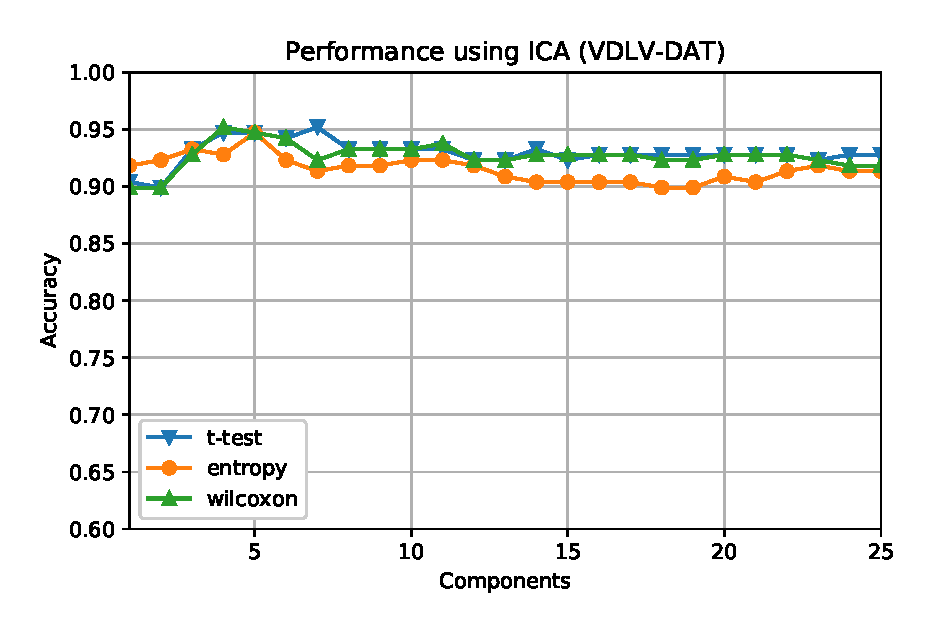
\includegraphics[width=0.49\linewidth]{Graphics/ch4/accuracyOP-ICA_vsN_comparison_VDLV-DAT.eps}\label{fig:VDLV-DAT-ICA-OP}}
	
	\caption[Performance at the operation point for the \acs{PKS} datasets, over the number of components.]{Performance of the proposed system using the two \ac{PKS} datasets: \ppmidat{}, \vdlndat{} and \vdlvdat{} at the operation point, and how they vary over the number of components used in the decomposition. } 
	\label{fig:accuracyOP-PKS}
\end{figure}

In this first case, the most evident result is the general performance of our system in the three datasets. It is clear that the system performs better when tested on \vdlvdat{} than when tested on \ppmidat{}, and both datasets outperform, \vdlndat{}. It is even clearer that when testing on \vdlvdat{}, the results are similar using any type of decomposition and selection criteria, with similar performance. We will discuss this issue in more detail later. 

The tendency of the performance at the operation point is similar to the average behaviour commented before. In general, there is an accuracy increasing in the first components (usually, between 5 and 10 depending on the decomposition) and then, the performance remains stable. Again, the combination of relative entropy selection and \vdlndat{} achieves striking results. For this dataset, the higher performance is obtained with more than 10 components ($c=14$), and shows higher variability than other datasets. 

Now we will focus on the specific performance values obtained at the operation point, that can be seen in Table~\ref{tab:featurePKS}. In this table we observe the differences in performance between datasets and also between \acp{CAD} using each decomposition strategy. 

\begin{table}
	\begin{tabularx}{\linewidth}{Xllccc}
		\toprule
		\tableheadline{DB} & \tableheadline{Dec.} & \tableheadline{Criterion} & \tableheadline{Accuracy} & \tableheadline{Sensitivity} & \tableheadline{Specificity}\\
		\toprule
		\multirow{7}{1.7cm}{\ppmidat{}} & \ac{VAF} & - & $ 0.800 \pm 0.071$ & $ 0.831 \pm 0.093$ & $0.747 \pm 0.112$ \\
		\cline{2-6}
		& \multirow{3}{*}{\ac{FA}} & t-test & $ 0.917 \pm 0.037 $ & $ 0.918 \pm 0.095 $ & $ 0.918 \pm 0.091 $ \\
		&  & entropy & $ 0.917 \pm 0.060 $ & $ 0.918 \pm 0.076 $ & $ 0.921 \pm 0.120 $ \\
		&  & wilcoxon & $ 0.912 \pm 0.056 $ & $ 0.927 \pm 0.098 $ & $ 0.889 \pm 0.102 $ \\
		\cline{2-6}
		& \multirow{3}{*}{\ac{ICA}} & t-test & $ 0.917 \pm 0.056 $ & $ 0.900 \pm 0.095 $ & $ 0.948 \pm 0.109 $ \\
		&  & entropy & $ 0.928 \pm 0.055 $ & $ 0.909 \pm 0.091 $ & $ 0.961 \pm 0.090 $ \\
		&  & wilcoxon & $ 0.912 \pm 0.070 $ & $ 0.909 \pm 0.100 $ & $ 0.920 \pm 0.118 $ \\
		\midrule
		\multirow{7}{1.7cm}{\vdlndat{}} & \ac{VAF} & - & $0.796 \pm 0.129 $ & $0.860 \pm 0.143 $ & $0.675 \pm 0.208 $ \\
		\cline{2-6}
		& \multirow{3}{*}{\ac{FA}} & t-test & $ 0.856 \pm 0.111 $ & $ 0.887 \pm 0.178 $ & $ 0.795 \pm 0.164 $ \\
		&  & entropy & $ 0.890 \pm 0.098 $ & $ 0.875 \pm 0.118 $ & $ 0.910 \pm 0.116 $ \\
		&  & wilcoxon & $ 0.864 \pm 0.070 $ & $ 0.916 \pm 0.114 $ & $ 0.780 \pm 0.183 $ \\
		\cline{2-6}
		& \multirow{3}{*}{\ac{ICA}} & t-test & $ 0.864 \pm 0.101 $ & $ 0.873 \pm 0.174 $ & $ 0.840 \pm 0.166 $ \\
		&  & entropy & $ 0.907 \pm 0.075 $ & $ 0.889 \pm 0.124 $ & $ 0.935 \pm 0.131 $ \\
		&  & wilcoxon & $ 0.873 \pm 0.108 $ & $ 0.859 \pm 0.181 $ & $ 0.890 \pm 0.151 $ \\
		\midrule
		\multirow{7}{1.7cm}{\vdlvdat{}} & \ac{VAF} & - & $ 0.918 \pm 0.062$ & $0.900 \pm 0.094$ & $ 0.926 \pm0.087$ \\
		\cline{2-6}
		& \multirow{3}{*}{\ac{FA}} & t-test & $ 0.957 \pm 0.063 $ & $ 0.910 \pm 0.094 $ & $ 0.973 \pm 0.065 $ \\
		&  & entropy & $ 0.952 \pm 0.037 $ & $ 0.940 \pm 0.066 $ & $ 0.964 \pm 0.064 $ \\
		&  & wilcoxon & $ 0.957 \pm 0.033 $ & $ 0.940 \pm 0.066 $ & $ 0.973 \pm 0.065 $ \\
		\cline{2-6}
		& \multirow{3}{*}{\ac{ICA}} & t-test & $ 0.952 \pm 0.037 $ & $ 0.940 \pm 0.066 $ & $ 0.964 \pm 0.064 $ \\
		&  & entropy & $ 0.947 \pm 0.045 $ & $ 0.940 \pm 0.066 $ & $ 0.955 \pm 0.076 $ \\
		&  & wilcoxon & $ 0.952 \pm 0.037 $ & $ 0.940 \pm 0.066 $ & $ 0.964 \pm 0.064 $ \\
		\bottomrule
	\end{tabularx}
	\caption[Performance values for the Parkinson's datasets]{Accuracy, sensitivity, specificity, and their standard deviation at the operation point for each method and its corresponding feature selection criterion, using three \protect\ac{PKS} datasets }
	\label{tab:featurePKS}
\end{table} 


In general, the systems using \ac{ICA} tend to perform slightly better than those using \ac{FA}, although the difference is small. There is little difference between selection criteria as well, although the combination of relative entropy and \ac{ICA} seems to work better, at least in the \ppmidat{} and \vdlndat{} (in \vdlvdat{} all combinations perform equally well). 


\FloatBarrier
\section{Discussion}
Now we will discuss the general behaviour of the selection and decomposition algorithm in the \ac{CAD} systems proposed and how they perform on the different diseases and databases. 

Our \ac{CAD} system performs reasonably well on the \ac{AD} datasets, where it achieves around 90\% accuracy, and more than 92\% sensitivity. This is achieved in both systems composed by \ac{FA} and \ac{ICA} regardless of the selection criterion chosen. The system outperforms the visual analysis estimated by means of \ac{VAF} \cite{Stoeckel04} in both cases. In \cite{Martinez201141} and \cite{Martinez-Murcia20129676}, the systems achieved better performance (up to 95.1\% accuracy) when using multivariate quadratic classifiers and \ac{ICA}, different from the \ac{SVC} used here. 

We have chosen to evaluate the system only on linear \acp{SVC} for two main reasons. First, it favours a side-by-side comparison between all methods applied to different datasets in this thesis. And second, linear \ac{SVC} has been proven to be better generalizable than other systems, even in environments where the small sample size is the norm \cite{Vapnik1997}. 

The selected areas on these \ac{CAD} systems correspond to the highlighted areas in Figure~\ref{fig:comparisonSelection_adnipet}, in the case of \adnipet{} dataset. 

\begin{figure}[bth]
	\myfloatalign
	\subfloat[$t$-test.]
	{\includegraphics[height=.25\textheight]{Graphics/ch4/ttest_map_adnipet.eps}\label{fig:ttest_map}}\quad
	\subfloat[\ac{KL} divergence.]
	{\includegraphics[height=.25\textheight]{Graphics/ch4/kl_map_adnipet.eps}\label{fig:kl_map}}\quad
	\subfloat[\ac{MWW} $U$-test.]
	{\includegraphics[height=.25\textheight]{Graphics/ch4/wilcoxon_map_adnipet.eps}\label{fig:wilcoxon_map}}
	\caption[Comparison between the different filtering methods in \adnipet{}.]{Comparison between the different filtering methods, and the regions selected by them, in the \adnipet{} dataset. }\label{fig:comparisonSelection_adnipet}
\end{figure}

In the \vdlnhmpao{} different areas are selected as we can see in Figure~\ref{fig:comparisonSelection_vdlnhmpao}. This is mainly due to a change in the modality that deserves to be analysed. 

\begin{figure}[bth]
	\myfloatalign
	\subfloat[$t$-test.]
	{\includegraphics[height=.25\textheight]{Graphics/ch4/ttest_map_vdln-hmpao.eps}\label{fig:ttest_map_vdlnhmpao}}\quad
	\subfloat[\ac{KL} divergence.]
	{\includegraphics[height=.25\textheight]{Graphics/ch4/kl_map_vdln-hmpao.eps}\label{fig:kl_map_vdlnhmpao}}\quad
	\subfloat[\ac{MWW} $U$-test.]
	{\includegraphics[height=.25\textheight]{Graphics/ch4/wilcoxon_map_vdln-hmpao.eps}\label{fig:wilcoxon_map_vdlnhmpao}}
	\caption[Comparison between the different filtering methods in \adnipet{}.]{Comparison between the different filtering methods, and the regions selected by them, in the \adnipet{} dataset. }\label{fig:comparisonSelection_vdlnhmpao}
\end{figure}

To have a more profound look at the selected regions in both modalities, we provide Table~\ref{tab:overlapVDLNAD}, where the AAL regions with an overlapping higher than 0.5 in any of the modalities and selection criteria are displayed. 

\begin{bigtable}
%	\centering
\begin{tabularx}{\textwidth}{Xcccccc}
	{} &\multicolumn{3}{c}{\adnipet{}}    & \multicolumn{3}{c}{\vdlnhmpao{}}         \\
	\cline{2-7}
	\tableheadline{Region} &    \tableheadline{entropy} & \tableheadline{t-test} & \tableheadline{wilcoxon} &  \tableheadline{entropy} & \tableheadline{t-test} & \tableheadline{wilcoxon} \\
	\midrule
Angular Gyrus (left)         &    \textbf{1.000} &    \textbf{1.000} &  \textbf{1.000} &      \textbf{1.000} &    \textbf{0.858} &  \textbf{1.000} \\
Angular Gyrus (right)         &    0.729 &    0.782 &  \textbf{0.809} &      \textbf{0.980} &    0.566 &  0.697 \\
Cingulum Posterior Part (left)   &    \textbf{1.000} &    \textbf{1.000} &  \textbf{1.000} &      0.589 &    0.509 &  0.773 \\
Cingulum Posterior Part (right)   &    \textbf{0.843} &    \textbf{0.852} &  0.791 &      0.524 &    0.228 &  0.442 \\
Cuneus (right)          &    0.173 &    0.121 &  0.188 &      \textbf{1.000} &    0.683 &  \textbf{0.857} \\
Fusiform Gyrus (left)        &    0.495 &    0.156 &  0.167 &      0.652 &    0.561 &  0.713 \\
Hippocampus (right)     &    \textbf{0.807} &    0.375 &  0.413 &      0.235 &    0.155 &  0.425 \\
Inferior Occipital Gyrus (left)   &    0.378 &    0.078 &  0.023 &      \textbf{1.000} &    \textbf{1.000} &  \textbf{1.000} \\
Inferior Occipital Gyrus (right)   &    0.380 &    0.080 &  0.011 &      \textbf{1.000} &    0.794 &  \textbf{0.930} \\
Inferior Parietal Lobule (right)    &    0.497 &    0.414 &  0.439 &      \textbf{1.000} &    0.339 &  0.477 \\
Inferior Temporal Gyrus (left)    &    0.748 &    0.350 &  0.495 &      0.676 &    0.561 &  0.735 \\
Middle Occipital Gyrus (left)   &    0.449 &    0.184 &  0.138 &      \textbf{1.000} &    \textbf{0.881} &  \textbf{1.000} \\
Middle Occipital Gyrus (right)   &    0.347 &    0.174 &  0.128 &      \textbf{0.861} &    0.642 &  0.770 \\
Middle Temporal Gyrus (left)    &    0.411 &    0.244 &  0.364 &      \textbf{0.952} &    0.635 &  \textbf{0.810} \\
Middle Temporal Gyrus (right)    &    0.594 &    0.234 &  0.326 &      \textbf{1.000} &    0.537 &  0.711 \\
Parahippocampal Gyrus (left) &    0.778 &    0.444 &  0.465 &      0.098 &    0.132 &  0.262 \\
Parahippocampal Gyrus (right) &    \textbf{0.917} &    0.276 &  0.316 &      0.233 &    0.159 &  0.311 \\
Precuneus (left)       &    0.322 &    0.429 &  0.463 &      0.708 &    0.485 &  0.660 \\
Precuneus (right)       &    0.311 &    0.375 &  0.409 &      0.770 &    0.469 &  0.644 \\
Superior Occipital Gyrus (right)   &    0.268 &    0.094 &  0.106 &      \textbf{0.955} &    0.600 &  0.736 \\
Supramarginal Gyrus (left)   &    0.195 &    0.156 &  0.183 &      0.627 &    0.561 &  0.762 \\
	\bottomrule
\end{tabularx}
\caption[Percentage of overlap between the selected areas by each method and the \acs{AAL} atlas regions.]{Percentage of overlap between the selected areas by each method and the \acs{AAL} atlas regions. For simplicity, overlapping values higher than 0.8 are displayed in bold.}
\label{tab:overlapVDLNAD}
\end{bigtable} 

In the case of the \vdlnhmpao{} dataset, the most interesting regions are located at the occipital lobe, the angular lobe and few of them in the temporal lobe. These are selected using almost any of the selection criteria. However, when using the \adnipet{} dataset, the only region with a significant overlapping is the angular gyrus, and other regions with a widely documented relation to \ac{AD} are highlighted \cite{Dubois2007,Claus1994}, such as the cingulum, hippocampus and parahippocampal gyrus. 

It is clearly noticeable that the relative entropy selection criterion focuses on many different regions, but it is the only one able to detect the hippocampus or parahippocampal gyrus in the \ac{PET} dataset, which other criteria ignore. It also focuses more on the different parts of the occipital lobe in the \ac{SPECT} dataset. This difference in the selected areas could lead to the different overall performance observed in Figures~\ref{fig:AD-AV-FA-ENTROPY-VSN}, \ref{fig:AD-AV-FA-ENTROPY-VSK}, \ref{fig:AD-AV-ICA-ENTROPY-VSN}, and \ref{fig:AD-AV-ICA-ENTROPY-VSK}.

For its part, wilcoxon and $t$-test often select similar regions. This can be due to their similarity under the normal distribution \cite{Fay10}, and leads to a higher performance in the systems in average and at the operation point (see Figures~\ref{fig:accuracyMeanFA-AD}, \ref{fig:accuracyMeanICA-AD}, \ref{fig:accuracyOP-ADvsN} and \ref{fig:accuracyOP-AD}). From the selected regions, and since $t$-test and wilcoxon perform generally better, we can infer the more interesting regions for \ac{AD} classification. For the \adnipet{} dataset, these would be the angular lobes and the cingulum, whereas for the \vdlnhmpao{}, we can observe differences in the angular lobe and also all over the occipital lobe and parts of the temporal lobe. 

Regarding the decomposition method, there seems not to be any significant differences. Both \ac{ICA} and \ac{FA} perform similarly in both datasets, regardless of the noise contained in the images, although the differences with the baseline system are much higher in the case of the \vdlnhmpao{} dataset. This is perhaps due to the smoother nature of the \adnipet{}, in which several images from the same subject were averaged, and therefore, much of the noise was removed, whereas in the \vdlnhmpao{} images, the noise could be removed afterwards by discarding many of the lower-significance components. 

When applied to the \ac{PKS} datasets, the results differ from the \ppmidat{} and \vdlndat{} to the \vdlvdat{}. These databases differ in the number of subjects that they contain. Whereas in the former there are different subjects with \ac{PKS}, including \ac{SWEDD}, in the later we only have \ac{PD} and \ac{CTL} subjects, which makes the classification easier. 

This accuracy differences can be found throughout all figures and tables, although in general, the \vdlndat{} dataset has the lowest performance, while the \ppmidat{} and \vdlvdat{} behave similarly in average. 

When using \ac{FA} with the \ac{PKS} datasets, we observe a similar behaviour to that already seen with \ac{AD} datasets: there is little difference in performance when varying the number of selected voxels, except when using the relative entropy criterion. In this particular case, there is a rise in the average performance when increasing the number of selected voxels, which is more noticeable when using the VDLN-DAt dataset. 

For its part, there are more significant variations when increasing the number of components. Smaller $c$ values lead to a fast increase in performance up to a maximum. Depending on the selection criterion used, this value varies from $c=3$ when using the $t$-test to $c=14$ for the entropy criterion applied to \vdlndat{}. The optimal $c$ is usually located at $c\in [3,5]$ in most cases, as can be seen in Figure~\ref{fig:accuracyMeanFA-PKS}. A very similar behaviour is achieved when using the \ac{ICA} decomposition, as Figure~\ref{fig:accuracyMeanICA-PKS} shows.

In \ac{AD} we provided a table with the selected regions in both \ac{PET} and \ac{SPECT} modalities. Conversely, in DaTSCAN imaging, the selected regions are always in the striatum, and the smaller resolution of these images hardly reveals the underlying structures. The selected regions with either $t$-test or wilcoxon fundamentally cover the whole caudate, putamen and globus pallidus, and some external structures as well. However, the relative entropy criterion focus almost exclusively in the striatum, with a strong preference for the posterior part, and discards all other regions, introducing less noise. 

\begin{figure}[bth]
	\myfloatalign
	\subfloat[$t$-test.]
	{\includegraphics[height=.25\textheight]{Graphics/ch4/ttest_map_ppmi-dat.eps}\label{fig:ttest_map_ppmi-dat}}\quad
	\subfloat[\ac{KL} divergence.]
	{\includegraphics[height=.25\textheight]{Graphics/ch4/kl_map_ppmi-dat.eps}\label{fig:kl_map_ppmi-dat}}\quad
	\subfloat[\ac{MWW} $U$-test.]
	{\includegraphics[height=.25\textheight]{Graphics/ch4/wilcoxon_map_ppmi-dat.eps}\label{fig:wilcoxon_map_ppmi-dat}}
	\caption[Comparison between the different filtering methods in \ppmidat{}.]{Comparison between the different filtering methods, and the regions selected by them, in the \ppmidat{} dataset. }\label{fig:comparisonSelection_ppmidat}
\end{figure}

This is clearly seen in Figure~\ref{fig:accuracyOP-PKSvsN} where the performance around the operation point is displayed. Here, when looking at the \vdlndat{} dataset, the correlation between performance and number of selected voxels is more obvious. As can be seen in Table~\ref{tab:featurePKS}, in the two datasets where \ac{SWEDD} subjects are included the system which uses relative entropy achieves better results. However, in the \vdlvdat{}, where the system only involves \ac{PD} and \ac{CTL} subjects, the performance is very similar using all three selection criteria. 

When looking at the evolution of the performance with the number of selected components, (Figure~\ref{fig:accuracyOP-PKS}), the pattern observed in \ac{AD} holds for the \ppmidat{} and the \vdlvdat{} datasets. In these cases, maximum performance is obtained with a relatively small $c$ (between 4 and 8, depending on the decomposition algorithm). However, with the relative entropy criterion, the \vdlndat{} still needs a higher number (more than 10) to reach the operation point. 

All these differences in behaviour could be due to a higher variability in \vdlndat{}, compared to the other two datasets. The number of components needed, especially in \ac{FA}, points to a more complex decomposition of those images. The sources of variability in this dataset probably correspond to a higher proportion of \ac{SWEDD} subjects and the number of cuts used in the acquisition. The number of \ac{SWEDD} in \vdlndat{} is 30 for a total dataset of 148 patients, whereas in the \ppmidat{} dataset we only have 31 \ac{SWEDD} for 301 subjects. Furthermore, the number of cuts in the images of \vdlndat{} differs from one image to another, since they follow a common practice in which only the \acp{ROI} of the brain (the striatum) are acquired. 
